\chapter{Descripción del trabajo realizado}

El presente capítulo describe el proceso de desarrollo e integración de la solución propuesta para el sistema de monitoreo y análisis de técnicas de modulación y demodulación implementado en el proyecto. Se abordan las principales decisiones de ingeniería adoptadas durante la construcción de la solución, considerando aspectos asociados al procesamiento digital de señales, integración hardware/software, comunicación de datos, modularidad y restricciones propias del entorno utilizado.

Inicialmente, se presenta una descripción general de la arquitectura de la solución y de la interacción entre sus principales componentes funcionales. Posteriormente, se describe el proceso seguido para el desarrollo de cada uno de los objetivos específicos del proyecto, enfatizando los criterios técnicos considerados durante la implementación y refinamiento progresivo del sistema. Finalmente, se realiza un análisis de los resultados obtenidos a partir del comportamiento funcional de la solución.

\section{Descripción de la arquitectura de la solución}

La solución propuesta se estructuró a partir de una arquitectura modular orientada a separar las principales responsabilidades funcionales del sistema, incluyendo adquisición de entradas, procesamiento de señales, transmisión de datos y visualización de información. Esta organización permitió distribuir el procesamiento entre el sistema embebido y la aplicación de monitoreo, facilitando la integración entre ambos entornos y manteniendo una estructura de funcionamiento más organizada y escalable.

La Figura \ref{fig:arquitectura} presenta la arquitectura general de la solución propuesta y la interacción existente entre los principales módulos funcionales del sistema.

\begin{figure}[H]
\centering
\resizebox{\textwidth}{!}{
    \shorthandoff{<>}
    \begin{tikzpicture}[
    >=Stealth,
    arrow/.style={->, thick},
    dashedbox/.style={
        draw,
        dashed,
        thick,
        rounded corners=4pt
    }
]

% ==================================================
% CAJA MODULADOR EMBEBIDO
% ==================================================

\node[dashedbox, minimum width=4cm, minimum height=4cm] (embeddedbox) at (-3,2.8)
{};

\node at (-3,5.2)
{
\small \textbf{Dispositivo Modulador}
};



% ==================================================
% CONTROLES ANALOGICOS
% ==================================================

\node (controls) at (-3,2.8)
{

\includegraphics[width=1.5cm]{fig/modulator.png}
};

\node[align=center] at (-3,3.8)
{
\scriptsize \textbf{Controladora}
};

% ==================================================
% CAJA SISTEMA EMBEBIDO
% ==================================================

\node[dashedbox, minimum width=10cm, minimum height=8.6cm] (embeddedbox) at (4.8,0.5)
{};

\node at (5,5.2)
{
\small \textbf{Sistema Embebido (Microcontrolador)}
};

% ==================================================
% GESTION DE ENTRADAS
% ==================================================

\node (inputs) at (1.3,2.8)
{

\includegraphics[width=1.4cm]{fig/input.png}
};

\node[align=center] at (1.3,3.7)
{
\scriptsize \textbf{Gestor de}\\[-7pt]
\scriptsize \textbf{entradas}
};

% ==================================================
% GENERADOR DE SEÑALES
% ==================================================

\node (generator) at (1.3,0)
{

\includegraphics[width=1.4cm]{fig/signal.png}
};

\node[align=center] at (1.3,-0.9)
{
\scriptsize \textbf{Generador de}\\[-7pt]
\scriptsize \textbf{señales}
};

% ==================================================
% MODULO PROCESAMIENTO
% ==================================================

\node (processing) at (5.2,0)
{

\includegraphics[width=1.8cm]{fig/chip.png}
};

\node[align=center] at (5.2,1.3)
{
\scriptsize \textbf{Módulo de}\\[-7pt]
\scriptsize \textbf{Procesamiento}
};

% ==================================================
% ALGORITMOS
% ==================================================

\node (algorithms) at (5.2,-2.5)
{

\includegraphics[width=1.4cm]{fig/algorithm.png}
};

\node[align=center] at (5.2,-3.5)
{
\scriptsize \textbf{Algoritmos}
};

% ==================================================
% MODULO ENVIO
% ==================================================

\node (data) at (8,0)
{

\includegraphics[width=1.6cm]{fig/database.png}
};

\node[align=center] at (8,-1.1)
{
\scriptsize \textbf{Módulo de envío}\\[-7pt]
\scriptsize \textbf{de datos}
};

% ==================================================
% SERIAL
% ==================================================

\node (serial) at (11.2,0)
{

\includegraphics[width=1.5cm]{fig/serial.png}
};

\node[align=center] at (11.2,-0.9)
{
\scriptsize \textbf{Módulo de}\\[-7pt]
\scriptsize \textbf{transmisión serial}
};

% ==================================================
% APP BOX
% ==================================================

\node[dashedbox, minimum width=6cm, minimum height=6cm] (appbox) at (15.7,0.8)
{};

\node at (15.7,4.2)
{
\small \textbf{App de Monitoreo}
};

% ==================================================
% CONFIG
% ==================================================

\node (config) at (15,2.8)
{

\includegraphics[width=1.5cm]{fig/config.png}
};

\node[align=center] at (15,1.8)
{
\scriptsize \textbf{Módulo de }\\[-7pt]
\scriptsize \textbf{Configuración}
};

% ==================================================
% RX
% ==================================================

\node (rx) at (14.3,0)
{

\includegraphics[width=1.5cm]{fig/reconstruct.png}
};

\node[align=center] at (14.3,-1.2)
{
\scriptsize \textbf{Reconstrucción y}\\[-7pt]
\scriptsize \textbf{recepción de datos}
};

% ==================================================
% VISUALIZACION
% ==================================================

\node (visual) at (17,0)
{

\includegraphics[width=1.5cm]{fig/pc.png}
};

\node[align=center] at (17,-1.2)
{
\scriptsize \textbf{Módulo de}\\[-7pt]
\scriptsize \textbf{Visualización}
};

% ==================================================
% FLECHAS PRINCIPALES
% ==================================================

\draw[arrow] (controls.east) -- (inputs.west);

\draw[arrow] (inputs.south) -- (generator.north);

\draw[arrow] (generator.east) -- (processing.west);

\draw[arrow] (algorithms.north) -- (processing.south);

\draw[arrow] (processing.east) -- (data.west);

\draw[arrow] (data.east) -- (serial.west);

\draw[arrow] (serial.east) -- (rx.west);

\draw[arrow] (rx.east) -- (visual.west);

% ==================================================
% CONFIGURACION
% ==================================================
\draw[arrow] (config.west) -- (inputs.east);

\draw[arrow]
(visual.north)
|- (config.east);



\end{tikzpicture}
    \shorthandon{<>}
}
\caption{Diagrama de arquitectura de la solución. Fuente: Elaboración propia.}
\label{fig:arquitectura}
\end{figure}

A nivel general, la arquitectura se compone de un dispositivo modulador basado en controles analógicos, un sistema embebido encargado del procesamiento principal de señales, un mecanismo de transmisión serial para el intercambio de información y una aplicación de monitoreo orientada a la reconstrucción, visualización y configuración del sistema. Dentro del sistema embebido se estableció una separación funcional entre los módulos de gestión de entradas, generación de señales, procesamiento de modulación y demodulación, integración de algoritmos y empaquetamiento de datos, permitiendo desacoplar las diferentes responsabilidades asociadas al flujo de procesamiento.

De manera complementaria, la aplicación de monitoreo se estructuró mediante módulos independientes de recepción y reconstrucción de datos, visualización de señales y configuración general del sistema, permitiendo mantener separadas las tareas asociadas al procesamiento gráfico, interpretación de información y control operativo.

\section{Descripción del proceso de solución}

A partir de la arquitectura definida para la solución propuesta, el proceso de desarrollo del sistema se orientó a la integración progresiva de los distintos componentes funcionales. A continuación, se describe el desarrollo realizado para cada uno de estos componentes, considerando las principales decisiones técnicas asociadas al sistema embebido, el procesamiento de señales, la comunicación de datos y la aplicación de monitoreo implementada para el proyecto.


\label{sec:adaptacion}
\subsection{Adaptación de los algoritmos al entorno embebido}

La adaptación de los algoritmos de modulación y demodulación al entorno embebido representa uno de los principales retos técnicos de la solución propuesta, debido a que las técnicas implementadas deben mantener funcionamiento continuo bajo restricciones asociadas a procesamiento, memoria, sincronización temporal y transmisión serial de datos. En este escenario, el problema no se limita únicamente a ejecutar ecuaciones de modulación y demodulación, sino a reorganizar las técnicas de procesamiento para mantener estabilidad operativa dentro de una arquitectura computacionalmente limitada.

\subsubsection{Selección de la plataforma embebida}

La selección de la plataforma embebida condiciona directamente la complejidad matemática permitida, la organización del procesamiento y la viabilidad temporal del sistema. Bajo este criterio, la plataforma seleccionada debe proporcionar capacidad suficiente para ejecutar procesamiento digital básico de señales, transmisión serial continua y adquisición de entradas analógicas, manteniendo simultáneamente bajo costo y simplicidad de integración.

La Tabla \ref{tab:placas_embebidas} presenta una comparación entre algunas de las plataformas consideradas durante esta etapa, utilizando información proveniente de las especificaciones oficiales de cada fabricante \cite{raspberrypiPicoDocs}.

\begin{table}[H]
\centering
\caption{Comparación entre plataformas embebidas consideradas.}
\label{tab:placas_embebidas}
\begin{tabular}{|>{\centering\arraybackslash}p{3.3cm}|>{\centering\arraybackslash}p{2.5cm}|>{\centering\arraybackslash}p{1.8cm}|>{\centering\arraybackslash}p{1.5cm}|>{\centering\arraybackslash}p{2.5cm}|>{\centering\arraybackslash}p{1.5cm}|}
\hline
\textbf{Plataforma} &
\textbf{Frecuencia} &
\textbf{RAM} &
\textbf{GPIO} &
\textbf{USB} &
\textbf{Costo aprox.} \\ \hline

Arduino Uno &
16 MHz &
2 kB &
14 &
USB Serial &
\$20 \\ \hline

Raspberry Pi Pico &
133 MHz &
264 kB &
26 &
USB CDC &
\$4 \\ \hline

ESP32 &
240 MHz &
520 kB &
34 &
USB-UART &
\$8 \\ \hline
\end{tabular}
\end{table}

En primera instancia, la plataforma Arduino Uno presenta restricciones importantes asociadas tanto a memoria como a capacidad de procesamiento para mantener generación, modulación, demodulación y transmisión continua de señales dentro de un mismo flujo operativo. La limitada cantidad de memoria SRAM disponible restringe significativamente el manejo simultáneo de buffers de señal, estructuras temporales de procesamiento y paquetes de transmisión serial, mientras que la frecuencia de operación del microcontrolador introduce limitaciones adicionales sobre la continuidad temporal requerida por el sistema. Bajo estas condiciones, la ejecución concurrente de procesos puede comprometer la estabilidad general del sistema.

Por otro lado, aunque ESP32 proporciona mayores capacidades computacionales y una cantidad superior de memoria disponible, gran parte de su arquitectura se orienta hacia aplicaciones IoT y comunicación inalámbrica. Esto incorpora subsistemas y mecanismos de conectividad que no aportan ventajas directas para el problema abordado, pero sí aumentan la complejidad general de integración, configuración y administración del entorno embebido. Adicionalmente, parte del enfoque de la solución consiste en mantener una arquitectura computacional relativamente simple, donde el procesamiento digital y la sincronización temporal de señales representen el núcleo principal del sistema.

Seguidamente, la Raspberry Pi Pico representa una alternativa más balanceada entre capacidad computacional, disponibilidad de periféricos y costo de implementación. La plataforma proporciona capacidad suficiente para mantener procesamiento continuo de señales, lectura simultánea de entradas analógicas y transmisión serial estructurada sin incorporar complejidad adicional asociada a conectividad externa o subsistemas no requeridos. Adicionalmente, la integración directa de comunicación USB, la disponibilidad de GPIO suficientes para interacción física y la compatibilidad con MicroPython favorecen una arquitectura más unificada entre el entorno embebido y el sistema de monitoreo desarrollado.

Luego de evaluar las opciones disponibles, la Raspberry Pi Pico es la plataforma embebida seleccionada para el desarrollo de la solución propuesta, esta placa utiliza como núcleo principal el microcontrolador RP2040, cuyas características técnicas relevantes se presentan en la Tabla \ref{tab:rp2040_specs} \cite{raspberrypiPicoDocs}.

\begin{table}[H]
\centering
\caption{Características técnicas relevantes del RP2040.}
\label{tab:rp2040_specs}

\resizebox{0.55\textwidth}{!}{
\begin{tabular}{|p{5cm}|p{6cm}|}
\hline
\textbf{Característica} & \textbf{Descripción} \\ \hline
Arquitectura & Dual-Core Arm Cortex-M0+ \\ \hline
Frecuencia máxima & Hasta 133 MHz \\ \hline
Memoria SRAM & 264 kB \\ \hline
Memoria Flash & Externa mediante QSPI \\ \hline
GPIO disponibles & 26 GPIO multipropósito \\ \hline
Entradas ADC & 3 canales de 12 bits \\ \hline
Comunicación USB & USB 1.1 con soporte CDC \\ \hline
Lenguajes soportados & C/C++ y MicroPython \\ \hline
\end{tabular}
}

\end{table}

A pesar de que la Raspberry Pi Pico representa la alternativa más adecuada para los requerimientos del sistema, el entorno embebido continúa imponiendo restricciones importantes sobre la complejidad matemática permitida durante la ejecución continua del procesamiento. Las capacidades computacionales y de memoria del RP2040 limitan el uso de bibliotecas orientadas a procesamiento numérico intensivo, como NumPy o SciPy, debido a sus requerimientos de memoria y estructuras vectorizadas. Esta restricción obliga a apoyarse principalmente en operaciones aritméticas básicas, procesamiento secuencial y estructuras matemáticas simplificadas, condicionando a su vez las decisiones de diseño algorítmico que se abordarán en las seccionessiguientes.

\subsubsection{Integración física del modulador}

Luego de seleccionar la plataforma embebida, se requiere definir un circuito que permita poner a disposición una estructura física mínima compuesta por elementos electrónicos que faciliten interactuar dinámicamente con las técnicas que se ejecutarán en el embebido. Bajo este criterio, el sistema se construye utilizando una estructura compuesta por la Raspberry Pi Pico, tres potenciómetros y un interruptor.

La Figura \ref{fig:pico_schematic} presenta el esquema general de conexión utilizado para la construcción del modulador físico.

\begin{figure}[H]
    \centering
    \resizebox{0.65\textwidth}{!}{
    
\definecolor{c3v3}{RGB}{0,90,200}
\definecolor{cgnd}{RGB}{20,135,30}
\definecolor{csig}{RGB}{160,0,0}

\begin{circuitikz}[
    american,
    scale      = 1.0,
    transform shape,
    line width = 0.65pt,
    font       = \small,
]

% ════════════════════════════════════════════════════════════════
%  LAYOUT
%
%  Strategy: pots are vertical, mirror=wiper exits RIGHT.
%  Wiper signal wire: goes right (offset from pot x), then drops
%  to the Pico pin — the pin is at the SAME x as the wiper wire,
%  so there is NO horizontal bottom segment and NO box artifact.
%
%  Pot positions (x of pot body):
%    Pot1  x=4.5    Wiper exits to x=5.3   Pico ADC pin at x=5.3
%    Pot2  x=7.5    Wiper exits to x=8.3   Pico ADC pin at x=8.3
%    Pot3  x=10.5   Wiper exits to x=11.3  Pico ADC pin at x=11.3
%
%  GND connections (left terminal of pot with mirror):
%    all on pot x (4.5 / 7.5 / 10.5) → GND rail below
%
%  3V3 connections (right terminal = top):
%    all on pot x → 3V3 rail above
%
%  Pico box:  (0,0)–(16,3)
%  Top pin stubs:
%    3V3     x=1.8
%    GP28_A2 x=5.3
%    GP27_A1 x=8.3
%    GP26_A0 x=11.3
%    GP16    x=14.0
%  Bottom GND: x=8.0
%
%  3V3 rail: y=9.8  x=1.8..11.8  (blue)
%  GND rail: y=-2.0 x=0.5..14.8  (green)
% ════════════════════════════════════════════════════════════════

% ── PICO BOX ────────────────────────────────────────────────────
\draw[thick, rounded corners=4pt]
    (0,0) rectangle (16,3);
\node[align=center] at (8,1.5)
    {\normalsize\bfseries Raspberry Pi Pico};

% Top pin stubs  (y=3 → y=3.35)
\foreach \x/\lbl in {
    1.8/{3V3},
    5.3/{GP28\_A2},
    8.3/{GP27\_A1},
    11.3/{GP26\_A0},
    14.0/{GP16}
}{
    \draw (\x,3) -- (\x,3.35);
    \node[above, font=\ttfamily\scriptsize, rotate=60, anchor=west]
        at (\x,3.3) {\lbl};
}

% Bottom GND stub
\draw (8,0) -- (8,-0.35);
\node[below, font=\ttfamily\scriptsize] at (8,-0.35) {GND};

% Cosmetic side pins
\foreach \y in {0.4,0.9,1.4,1.9,2.4,2.9}{
    \draw (0,\y)  -- (-0.22,\y);
    \draw (16,\y) -- (16.22,\y);
}

% ── 3V3 RAIL  (blue) ────────────────────────────────────────────
\draw[c3v3, thick]
    (1.8,3.35) -- (1.8,9.8) -- (10.5,9.8);

% Taps to each pot top pin (y=8.8)  — pot x = 4.5, 7.5, 10.5
\foreach \x in {4.5,7.5,10.5}{
    \draw[c3v3, thick] (\x,9.8) -- (\x,8.8);
    \fill[c3v3] (\x,9.8) circle (2.2pt);
}

% ── GND RAIL  (green) ───────────────────────────────────────────
\draw[cgnd, thick]
    (8,-0.35) -- (8,-2.0)
    (4.5,-2.0) -- (14.5,-2.0);
\node[ground, cgnd] at (8,-2.0) {};

% Taps from GND rail up to pot bottom pins (y=5.2) — pot x = 4.5, 7.5, 10.5
\foreach \x in {4.5,7.5,10.5}{
    \draw[cgnd, thick] (\x,-2.0) -- (\x,5.2);
    \fill[cgnd] (\x,-2.0) circle (2.2pt);
}

% GND tap for switch at x=14.5
\draw[cgnd, thick] (14.5,-2.0) -- (14.5,6.5);
\fill[cgnd] (14.5,-2.0) circle (2.2pt);

% ── POTENTIOMETERS  (vertical, mirror → wiper exits right) ──────
%  bottom = GND (left terminal with mirror)
%  top    = 3V3 (right terminal with mirror)

% ---- Pot 1  (ADC2 / GP28) ----
\draw (4.5,5.2) to[pR, n=p1, mirror] (4.5,8.8);
\node[left=4pt, font=\footnotesize\bfseries, align=right] at (4.1,8.0)
    {Pot 1 \\ 10\,k$\Omega$};

% Wiper → right to x=5.3 (same as ADC pin) → straight down to Pico
\draw[csig, thick]
    (p1.wiper) -- (5.3,6.85) -- (5.3,3.35);
\fill[csig] (5.3,3.35) circle (2pt);

% ---- Pot 2  (ADC1 / GP27) ----
\draw (7.5,5.2) to[pR, n=p2, mirror] (7.5,8.8);
\node[left=4pt, font=\footnotesize\bfseries, align=right] at (7.1,8.0)
    {Pot 2 \\ 10\,k$\Omega$};

\draw[csig, thick]
    (p2.wiper) -- (8.3,6.85) -- (8.3,3.35);
\fill[csig] (8.3,3.35) circle (2pt);

% ---- Pot 3  (ADC0 / GP26) ----
\draw (10.5,5.2) to[pR, n=p3, mirror] (10.5,8.8);
\node[left=4pt, font=\footnotesize\bfseries, align=right] at (10.1,8.0)
    {Pot 3 \\ 10\,k$\Omega$};

\draw[csig, thick]
    (p3.wiper) -- (11.3,6.85) -- (11.3,3.35);
\fill[csig] (11.3,3.35) circle (2pt);

% ── SWITCH S1  (SPST-NO) ────────────────────────────────────────
% GP16 (x=14.0, y=3.35) → wire up → bottom of S1
% Top of S1 → GND at x=14.5

\draw[thick] (14.0,3.35) -- (14.0,4.8);
\draw (14.0,4.8) to[spst] (14.0,6.5);

% Top terminal → GND rail (green) via x=14.5
\draw[cgnd, thick] (14.0,6.5) -- (14.5,6.5);
% (14.5 already goes down to GND rail)

\node[right=4pt, font=\footnotesize\bfseries] at (14.0,5.65) {S1};
\node[right=4pt, font=\footnotesize\itshape]  at (14.0,5.05) {AM / ASK};

\end{circuitikz}

    }
    \caption{Esquemático general del módulo físico de control utilizado por el sistema embebido.}
    \label{fig:pico_schematic}
\end{figure}

Los tres potenciómetros se conectan a los canales ADC disponibles del RP2040 (GPIO 26, 27 y 28), mientras que el interruptor se conecta a un pin GPIO configurado con resistencia de pull-up interna. Esta configuración permite al sistema embebido adquirir de forma continua tres valores analógicos normalizados en el rango $[0,1]$ y un estado binario de selección de técnica, utilizando únicamente periféricos nativos del microcontrolador sin requerir componentes externos adicionales.

\subsubsection{Adaptación de la técnica AM}

La adaptación de la técnica AM al entorno embebido representa una decisión crítica dentro del diseño de la solución, debido a que esta técnica puede implementarse con distintos niveles de complejidad matemática y, por tanto, con diferentes implicaciones sobre precisión, carga computacional y estabilidad temporal. Bajo este escenario, el problema no consiste únicamente en aplicar la ecuación clásica de modulación, sino en definir hasta qué punto resulta conveniente trasladar al microcontrolador una representación más completa del proceso de modulación y demodulación, considerando que el sistema debe ejecutar simultáneamente generación de señales, lectura de parámetros físicos, procesamiento continuo de bloques y transmisión serial hacia la aplicación de monitoreo.

Para la etapa de modulación AM se consideran dos enfoques principales. El primero corresponde a una implementación con mayor acondicionamiento matemático sobre la señal, incorporando una etapa de normalización, control más estricto de amplitud y ajustes adicionales sobre la señal de información antes de aplicar la portadora. Bajo esta alternativa, la señal de información $m[n]$ no se utiliza directamente, sino que es previamente acondicionada para mantener su amplitud dentro de un rango controlado:

\begin{equation}
m_a[n] = \frac{m[n]}{\max(|m[n]|)}
\label{eq:am_normalizacion_completa}
\end{equation}

Posteriormente, la señal modulada se obtiene mediante:

\begin{equation}
s[n] = A_c \left(1 + \mu m_a[n]\right)\cos(2\pi f_c nT_s)
\label{eq:am_mod_completa}
\end{equation}

donde $A_c$ representa la amplitud de la portadora, $\mu$ el índice de modulación, $f_c$ la frecuencia de portadora y $T_s$ el periodo de muestreo.

Esta alternativa proporciona un mayor control matemático sobre la amplitud de la señal modulada y reduce el riesgo de sobre-modulación o saturación frente a variaciones de amplitud de la señal de entrada. Adicionalmente, el uso de una señal previamente acondicionada favorece un comportamiento más estable de la envolvente y contribuye a mantener una reconstrucción más controlada durante la demodulación.

Sin embargo, este enfoque también incrementa considerablemente la carga de procesamiento dentro del entorno embebido. La normalización requiere recorrer bloques completos de muestras, calcular máximos, realizar divisiones sucesivas y mantener controles adicionales sobre el rango dinámico de la señal. Aunque estas operaciones resultan relativamente comunes en entornos de simulación o procesamiento DSP convencional, su ejecución continua dentro de MicroPython sobre un microcontrolador implica un aumento significativo en el costo computacional. En consecuencia, esta alternativa prioriza precisión matemática y acondicionamiento de señal, pero aproxima simultáneamente al sistema embebido a sus límites de procesamiento.

Como alternativa, la modulación puede representarse mediante una formulación discreta simplificada orientada a preservar únicamente el comportamiento funcional esencial de AM. En este contexto, la señal de información es generada directamente dentro de un rango previamente controlado, eliminando la necesidad de incorporar una etapa adicional de normalización dinámica por bloque. La modulación se expresa como:

\begin{equation}
s[n] = \left(1 + \mu m[n]\right)c[n]
\label{eq:am_mod_embebido}
\end{equation}

con:

\begin{equation}
c[n] = \cos(2\pi f_c nT_s)
\label{eq:am_portadora}
\end{equation}

Esta formulación reduce el procesamiento requerido a operaciones elementales de suma, multiplicación y evaluación trigonométrica de la portadora. La principal ventaja de este enfoque corresponde a la disminución significativa de la carga computacional asociada al procesamiento continuo. Debido a que la arquitectura elimina etapas adicionales de acondicionamiento y control dinámico, el microcontrolador dispone de mayor margen operativo para sostener simultáneamente el procesamiento interno, la transmisión serial y la actualización continua de parámetros del sistema.

La diferencia entre ambas alternativas radica en que, la primera estrategia favorece la precisión matemática, control de amplitud y estabilidad formal sobre la señal modulada, pero incrementa el procesamiento requerido por bloque, mientras que, la segunda reduce parte de ese acondicionamiento adicional y prioriza simplicidad operativa y estabilidad temporal dentro del entorno embebido, conservando al mismo tiempo el comportamiento funcional fundamental de la técnica.

Considerando que la señal de información utilizada dentro del sistema no proviene de una fuente externa arbitraria, sino que es generada internamente mediante parámetros controlados por el propio sistema, la arquitectura final se orienta hacia la formulación discreta simplificada. Esta decisión permite mantener una representación adecuada del fenómeno de modulación AM sin incorporar etapas adicionales de procesamiento que incrementen innecesariamente la carga computacional del microcontrolador. En consecuencia, el enfoque seleccionado proporciona un balance más adecuado entre representatividad funcional, estabilidad temporal y viabilidad computacional dentro del entorno embebido.

La etapa de demodulación introduce una segunda decisión crítica asociada al mecanismo de recuperación de la señal de información. En este caso se consideran dos alternativas técnicamente viables: la demodulación por envolvente y la demodulación coherente. Ambos enfoques permiten recuperar la información contenida en la señal AM, aunque presentan diferencias importantes respecto a sensibilidad, complejidad y compatibilidad con la arquitectura general del sistema.

La primera alternativa corresponde a la demodulación por envolvente. En este enfoque, la señal modulada es transformada en una señal positiva que permita aproximar su envolvente y posteriormente aplicar filtrado pasa bajos para recuperar la señal de información. De forma simplificada, este proceso puede representarse mediante:

\begin{equation}
e[n] = |s[n]|
\label{eq:am_envolvente_abs}
\end{equation}

seguido por:

\begin{equation}
\hat{m}[n] = LPF\{e[n]\}
\label{eq:am_envolvente_lpf}
\end{equation}

La principal ventaja de esta estrategia consiste en que elimina la necesidad de utilizar una referencia local de portadora durante la recuperación. Esto simplifica parcialmente la arquitectura de detección y reduce la dependencia sobre mecanismos de sincronización explícita entre modulación y demodulación. Adicionalmente, la detección por envolvente mantiene una relación directa con arquitecturas clásicas de recuperación AM y permite implementar un proceso conceptualmente sencillo.

No obstante, este enfoque también introduce limitaciones importantes dentro del contexto del proyecto. La calidad de recuperación depende considerablemente del comportamiento de la envolvente detectada y del filtrado posterior aplicado sobre la señal. Variaciones sobre amplitud, componentes residuales de alta frecuencia o cambios sobre el índice de modulación pueden afectar la estabilidad de la envolvente estimada y generar distorsión sobre la señal recuperada. En consecuencia, aunque esta alternativa reduce parcialmente la complejidad asociada a sincronización, traslada gran parte del problema hacia el diseño del filtrado y la estabilidad de la detección de amplitud.

La segunda alternativa corresponde a la demodulación coherente. Bajo este enfoque, la señal modulada es multiplicada directamente por una referencia local de portadora equivalente a la utilizada durante la modulación:

\begin{equation}
y[n] = s[n] \cdot c[n]
\label{eq:am_demod_coherente}
\end{equation}

Sustituyendo la señal modulada en la ecuación \eqref{eq:am_demod_coherente}, se obtiene:

\begin{equation}
y[n] = \left(1 + \mu m[n]\right)c^2[n]
\label{eq:am_demod_coherente_expandida}
\end{equation}

Debido a que esta multiplicación genera simultáneamente componentes de baja y alta frecuencia, la señal resultante requiere una etapa posterior de filtrado pasa bajos:

\begin{equation}
\hat{m}[n] = LPF\{y[n]\}
\label{eq:am_demod_coherente_lpf}
\end{equation}

La principal ventaja de este enfoque corresponde al mayor control matemático que proporciona sobre el proceso de recuperación. Debido a que la detección utiliza una referencia conocida de portadora, la reconstrucción de señal resulta menos dependiente del comportamiento instantáneo de la envolvente y mantiene una recuperación más estable frente a variaciones moderadas de amplitud.

Adicionalmente, dentro de la arquitectura propuesta, la portadora utilizada durante la modulación es generada internamente por el propio sistema embebido. Esto permite reutilizar directamente la referencia necesaria para la detección sin incorporar mecanismos complejos adicionales de sincronización, lo cual favorece la compatibilidad de este enfoque con la estructura general del sistema.

Sin embargo, la demodulación coherente también incrementa la cantidad de operaciones requeridas durante el procesamiento continuo. La necesidad de realizar multiplicaciones adicionales por muestra y mantener la referencia de portadora implica un costo computacional mayor respecto a una detección por envolvente simple. Bajo este escenario, la decisión no depende únicamente del método de recuperación seleccionado, sino también del tipo de filtrado que el sistema puede sostener sin comprometer la estabilidad temporal del procesamiento continuo.

Para la etapa de filtrado posterior se consideran igualmente dos alternativas. La primera consiste en utilizar filtros digitales de mayor selectividad frecuencial, capaces de proporcionar una reconstrucción más precisa de la señal recuperada. De forma general, esta alternativa puede representarse como:

\begin{equation}
\hat{m}[n] = \sum_{k=0}^{M} b_k y[n-k]
\label{eq:am_filtro_fir}
\end{equation}

donde $b_k$ representa los coeficientes del filtro y $M$ su orden.

La ventaja de este enfoque corresponde al mayor control sobre la respuesta frecuencial del sistema y a la posibilidad de mejorar la calidad de reconstrucción de la señal. Sin embargo, este tipo de filtros incrementa considerablemente la cantidad de multiplicaciones, sumas y almacenamiento temporal requeridos durante el procesamiento continuo, aumentando simultáneamente el consumo de memoria y tiempo de ejecución.

Como alternativa más ligera, la arquitectura propuesta incorpora un filtro pasa bajos recursivo de primer orden:

\begin{equation}
\hat{m}[n] = \hat{m}[n-1] + \alpha\left(y[n] - \hat{m}[n-1]\right)
\label{eq:am_lpf}
\end{equation}

donde $\alpha$ representa el coeficiente de suavizado asociado al filtro.

Aunque esta estructura no proporciona el mismo nivel de selectividad que un filtro digital de mayor orden, reduce considerablemente el costo computacional asociado al procesamiento continuo y únicamente requiere conservar el estado previo de la salida filtrada. La continuidad entre bloques consecutivos se preserva manteniendo el estado del filtro entre iteraciones del ciclo principal, evitando discontinuidades en la señal recuperada.

A partir de este análisis, la arquitectura final se orienta hacia una demodulación coherente complementada mediante un filtro pasa bajos recursivo de primer orden. Esta decisión permite evitar la alta dependencia de la detección por envolvente respecto al filtrado y comportamiento de amplitud, sin trasladar simultáneamente al microcontrolador una carga excesiva de procesamiento asociada a filtros digitales más complejos. En consecuencia, la solución seleccionada proporciona un balance adecuado entre estabilidad de recuperación, simplicidad matemática y viabilidad computacional dentro del entorno embebido.

\subsubsection{Adaptación de la técnica ASK/OOK}

La adaptación de la técnica ASK/OOK introduce un problema distinto al presente en AM, debido a que el sistema requiere generar información digital continua sin depender de almacenamiento extensivo de datos ni comunicación permanente con fuentes externas. Debido a esto, la principal dificultad no consiste únicamente en aplicar la ecuación de modulación digital, sino en definir cómo construir una señal binaria continua compatible con las restricciones computacionales presentes.

Una primera alternativa consiste en utilizar secuencias binarias precargadas dentro de memoria. Esto implica que la generación digital se basa en recorrer patrones previamente almacenados, simplificando parcialmente la arquitectura de generación de señal debido a que el sistema únicamente debe leer estados binarios previamente definidos, donde $b[n] \in \{0,1\}$.

La principal ventaja de esta estrategia corresponde a su simplicidad operacional. Debido a que los estados lógicos ya existen dentro de memoria, el procesamiento requerido para generar la señal digital resulta considerablemente bajo. Esto favorece la estabilidad temporal del sistema y reduce el costo computacional asociado a la generación continua de datos digitales.

Sin embargo, esta alternativa también introduce limitaciones importantes sobre escalabilidad y flexibilidad de la señal generada. Conforme aumenta el tamaño de las secuencias binarias utilizadas, también aumenta el uso de memoria requerido por el sistema embebido. Adicionalmente, la reutilización continua de patrones estáticos limita considerablemente la variabilidad de la señal y reduce la capacidad del sistema para representar comportamientos digitales más dinámicos. Debido a esto, el sistema prioriza simplicidad y estabilidad operativa, pero sacrifica flexibilidad y capacidad de generación autónoma de información digital.

Como segunda alternativa, se considera la generación pseudoaleatoria controlada mediante un valor de semilla (seed). En este enfoque, la señal digital no es almacenada explícitamente ni transmitida continuamente desde el exterior, sino generada matemáticamente dentro del propio entorno embebido utilizando estructuras ligeras de memoria y operaciones aritméticas simples.

La generación pseudoaleatoria puede representarse mediante una relación recursiva discreta:

\begin{equation}
r[n+1] = (a r[n] + c)\ \bmod\ M
\label{eq:ask_lcg}
\end{equation}

donde $r[n]$ corresponde al estado pseudoaleatorio interno, mientras que $a$, $c$ y $M$ representan constantes asociadas al generador.

La principal ventaja de esta estrategia corresponde a que permite construir patrones digitales reproducibles utilizando únicamente un estado interno reducido y operaciones matemáticas elementales. Esto elimina la necesidad de almacenar secuencias binarias extensas y mantiene simultáneamente independencia operativa respecto al sistema externo. Adicionalmente, el uso de una semilla permite controlar la generación de patrones y reproducir secuencias idénticas bajo las mismas condiciones de inicialización, lo cual resulta particularmente útil para análisis comparativos y validación de comportamiento.

Sin embargo, la generación pseudoaleatoria no representa directamente estados binarios. Debido a esto, la arquitectura requiere incorporar un mecanismo de decisión que transforme los valores pseudoaleatorios generados en estados lógicos discretos. Para resolver este problema, la señal digital se obtiene mediante una comparación contra un umbral de decisión:

\begin{equation}
b[n] =
\begin{cases}
1, & r[n] > \tau \\
0, & r[n] \leq \tau
\end{cases}
\label{eq:ask_threshold_embebido}
\end{equation}

donde $r[n]$ representa el valor pseudoaleatorio generado y $\tau$ el umbral de decisión.

Una vez obtenida la secuencia binaria, la modulación ASK/OOK se implementa mediante una relación directa entre el estado lógico y la portadora:

\begin{equation}
s[n] = b[n] \cdot c[n]
\label{eq:ask_mod_embebido}
\end{equation}

donde $b[n]$ corresponde a la señal binaria discreta y $c[n]$ a la portadora.

La utilización de esta formulación permite mantener una arquitectura matemática considerablemente más simple que otros esquemas de modulación digital más complejos. Debido a que la técnica únicamente requiere activar o desactivar la portadora dependiendo del estado lógico transmitido, el procesamiento asociado a la modulación se reduce principalmente a operaciones de comparación y multiplicación. Esto favorece considerablemente la estabilidad temporal del sistema y disminuye el costo computacional asociado al procesamiento continuo de señal dentro del entorno embebido.

La recuperación de señal digital introduce una segunda decisión crítica asociada al mecanismo de detección utilizado. Una primera alternativa corresponde a mecanismos avanzados de recuperación simbólica y sincronización digital. Bajo este enfoque, la detección incorpora estructuras orientadas a mantener alineamiento temporal continuo entre la señal recibida y el proceso de reconstrucción binaria, incluyendo recuperación de reloj, sincronización de símbolos y técnicas de detección digital más elaboradas.

Conceptualmente, este tipo de arquitecturas puede representarse mediante un proceso general de sincronización simbólica:

\begin{equation}
\hat{b}[k] = D\{s[n], \phi[n], T_b\}
\label{eq:ask_symbol_sync}
\end{equation}

donde $\phi[n]$ representa parámetros de sincronización temporal y $T_b$ el periodo simbólico asociado a cada bit.

La principal ventaja de esta estrategia corresponde al mayor nivel de robustez frente a ruido, desalineamiento temporal y variaciones sobre el comportamiento de la señal recibida. Debido a que el sistema mantiene control explícito sobre sincronización de símbolos y recuperación temporal, la detección binaria puede conservar mayor precisión bajo condiciones más complejas de transmisión.

Sin embargo, estos mecanismos introducen estructuras considerablemente más complejas para mantener sincronización continua entre la señal recibida y el proceso de detección. La recuperación simbólica requiere procesamiento temporal adicional, almacenamiento de estados internos y control más elaborado sobre el flujo de datos digitales. En consecuencia, aunque esta alternativa proporciona mayor robustez matemática y estabilidad sobre la detección, también incrementa significativamente la carga computacional y la complejidad del sistema.

Como alternativa, la arquitectura propuesta utiliza una estrategia coherente simplificada basada nuevamente en multiplicación directa entre la señal recibida y una portadora local, siguiendo el mismo principio matemático presentado en la ecuación \ref{eq:am_demod_coherente}. Posteriormente, la señal detectada se procesa mediante el mismo filtro pasa bajos recursivo de primer orden definido en la ecuación \ref{eq:am_lpf}. En este caso, la estructura no se utiliza para reconstruir una señal analógica continua, sino para suavizar la componente detectada antes de aplicar la decisión binaria. Esta reutilización del mismo esquema de filtrado permite mantener consistencia entre técnicas y reducir la complejidad de implementación dentro del entorno embebido.

Finalmente, la decisión lógica se obtiene mediante comparación contra un umbral:

\begin{equation}
b_d[n] =
\begin{cases}
1, & \hat{b}[n] > \tau \\
0, & \hat{b}[n] \leq \tau
\end{cases}
\label{eq:ask_decision}
\end{equation}

La principal ventaja de esta estrategia corresponde a que permite mantener una arquitectura considerablemente más ligera desde el punto de vista computacional. Debido a que la detección utiliza únicamente multiplicación directa, filtrado recursivo simple y comparación contra umbral, el sistema evita incorporar mecanismos avanzados de sincronización simbólica que podrían comprometer la estabilidad temporal del procesamiento continuo dentro del microcontrolador. Adicionalmente, dentro de la arquitectura propuesta, la portadora utilizada durante la modulación es generada internamente por el propio sistema embebido, lo que permite reutilizar directamente la referencia necesaria para la detección coherente sin requerir procesos adicionales de sincronización.

La diferencia entre ambas alternativas no corresponde a que una resulte técnicamente superior de forma absoluta, sino al balance entre robustez matemática y viabilidad computacional que cada una representa. Los mecanismos avanzados de sincronización digital ofrecen mayor precisión y tolerancia frente a desalineamiento temporal, pero incrementan considerablemente la complejidad del procesamiento embebido. Por otro lado, la estrategia coherente simplificada reduce parte de esa robustez adicional, pero mantiene una arquitectura considerablemente más estable y compatible con las restricciones reales del sistema.

\subsubsection{Integración de controles analógicos}

A partir de la estructura física presentada en la Figura \ref{fig:pico_schematic}, los periféricos analógicos del sistema se reutilizan como una interfaz de control común para las distintas técnicas implementadas. Por esta razón, los potenciómetros identificados como pot1, pot2 y pot3 adquieren una funcionalidad distinta dependiendo de la técnica activa dentro del sistema.

La Tabla \ref{tab:controles_analogicos} presenta la asignación funcional utilizada para cada técnica implementada.

\begin{table}[H]
\centering
\caption{Asignación de controles analógicos por técnica implementada.}
\label{tab:controles_analogicos}
\begin{tabular}{|>{\centering\arraybackslash}p{4cm}|>{\centering\arraybackslash}p{5cm}|>{\centering\arraybackslash}p{5cm}|}
\hline
\textbf{Control} & \textbf{AM} & \textbf{ASK/OOK} \\ \hline
pot1 & Frecuencia de mensaje & Valor de semilla \\ \hline
pot2 & Frecuencia de portadora & Frecuencia de portadora \\ \hline
pot3 & Índice de modulación $\mu$ & Umbral de decisión $\tau$ \\ \hline
\end{tabular}
\end{table}

La reutilización de la misma estructura física entre técnicas reduce complejidad de hardware y evita incorporar interfaces de control independientes para cada algoritmo implementado. Aunque cada parámetro adquiere un significado funcional distinto dependiendo de la técnica activa, la arquitectura de adquisición analógica permanece desacoplada de la lógica específica de modulación y demodulación.

\label{sec:flow_control}
\subsubsection{Manejo del flujo de datos}

La ejecución continua del sistema requiere mantener un flujo organizado de datos entre las distintas etapas internas de procesamiento, desde la generación de la señal hasta su posterior transmisión hacia la aplicación de monitoreo. En este contexto, la arquitectura debe permitir que la señal original, la señal modulada y la señal demodulada permanezcan temporalmente disponibles dentro del entorno embebido para conservar sincronización entre todas las etapas del proceso.

Para resolver este problema, la arquitectura se organiza mediante procesamiento por bloques, donde cada conjunto de muestras representa una unidad funcional completa de señal. Inicialmente se genera un bloque correspondiente a la señal original, el cual posteriormente es utilizado como entrada para la etapa de modulación. A partir de este bloque se construye una segunda representación asociada a la señal modulada y, seguidamente, una tercera representación correspondiente a la señal demodulada.

En lugar de sobrescribir continuamente cada etapa de procesamiento, la arquitectura conserva simultáneamente las tres versiones de la señal dentro de buffers independientes. Esto permite mantener alineación temporal entre las distintas representaciones y evita pérdidas de coherencia entre el proceso de generación, modulación y recuperación de señal.

Una vez completado el procesamiento interno del bloque, las tres etapas de señal son agrupadas dentro de un mismo frame serial estructurado para posteriormente ser transmitidas hacia el sistema de monitoreo.


\subsection{Desarrollo del sistema de visualización y monitoreo}


La implementación del sistema embebido requiere no solamente ejecutar los procesos de modulación y demodulación sobre el RP2040, sino también disponer de un mecanismo que permita observar continuamente el comportamiento de las señales procesadas durante la ejecución del sistema. Debido a esto, la visualización pasa a convertirse en un componente fundamental para verificar el funcionamiento de las técnicas implementadas y comparar simultáneamente la señal original, la modulada y la demodulada durante cada etapa del procesamiento.

A diferencia de un entorno de simulación, en donde el procesamiento y la visualización se ejecutaban dentro de un mismo entorno local, en este proyecto el procesamiento principal ocurre sobre un sistema embebido y la visualización se realiza en un entorno externo. Esto introduce la necesidad de transmitir continuamente información fuera del sistema embebido, donde posteriormente las señales van a ser reconstruidas y visualizadas.

Bajo este escenario, el sistema de monitoreo debe sostener adquisición continua de datos manteniendo simultáneamente estabilidad visual, sincronización temporal entre señales y capacidad de actualización durante la ejecución del sistema. Esto introduce restricciones asociadas al manejo continuo de información, latencia de actualización y sincronización temporal entre bloques transmitidos mediante comunicación serial.


\subsubsection{Diseño del módulo de visualización}

Conociendo que el sistema de monitoreo debe sostener visualización continua de múltiples señales durante la ejecución del sistema, el siguiente paso consiste en definir la arquitectura y las herramientas necesarias para construir una aplicación capaz de lograr este objetivo.

Uno de los aspectos importantes dentro de esta etapa consiste en definir el entorno de desarrollo utilizado para construir la aplicación de monitoreo. Considerando que el entorno embebido se encuentra basado sobre MicroPython, se prioriza mantener Python también como lenguaje principal para la aplicación. Esto permite conservar uniformidad tecnológica entre ambas partes del sistema, reduciendo simultáneamente complejidad asociada a la integración entre distintos lenguajes, manejo de estructuras heterogéneas y adaptación entre diferentes entornos de ejecución. Adicionalmente, Python proporciona un ecosistema particularmente conveniente para aplicaciones orientadas a procesamiento de señales y visualización científica, principalmente debido a la disponibilidad de librerías para comunicación serial, manejo eficiente de estructuras numéricas y construcción de interfaces gráficas.

Teniendo a Python como entorno principal, el siguiente paso consiste en seleccionar el framework gráfico y las herramientas de visualización capaces de sostener actualización continua de señales sin degradar significativamente el rendimiento del sistema. Debido a esto, se selecciona PyQt5 como framework principal para el desarrollo de la interfaz de monitoreo, principalmente por su integración con librerías orientadas a renderizado dinámico de información y su capacidad para construir aplicaciones gráficas organizadas alrededor de múltiples regiones funcionales.

A partir de esta arquitectura basada en PyQt5, inicialmente se considera reutilizar parte del enfoque de visualización utilizado en el proyecto antecesor a este, donde la representación gráfica se encontraba basada principalmente en Matplotlib. Sin embargo, aunque Matplotlib constituye una herramienta ampliamente utilizada para representación científica y análisis de datos, comienzan a observarse limitaciones importantes cuando el entorno de ejecución pasa de un escenario de simulación convencional hacia un sistema basado en adquisición continua de información externa.

A diferencia de un enfoque estático, donde las gráficas son actualizadas ocasionalmente o posterior al procesamiento, el sistema desarrollado requiere refresco continuo de múltiples señales mientras simultáneamente se reciben nuevos bloques de información mediante comunicación serial. Bajo este escenario, el problema deja de estar asociado únicamente a representar señales y pasa a involucrar restricciones relacionadas con frecuencia de actualización, estabilidad temporal, latencia de renderizado y manejo eficiente de buffers gráficos. Debido a esto, en la Tabla \ref{tab:mpl_vs_pyqtgraph} se realiza una comparación entre Matplotlib y PyQtGraph considerando los criterios mencionados.

\begin{table}[H]
\centering
\caption{Comparación entre Matplotlib y PyQtGraph para visualización continua}
\label{tab:mpl_vs_pyqtgraph}
\resizebox{0.65\textwidth}{!}{
\begin{tabular}{|p{4cm}|p{4cm}|p{4cm}|}
\hline
\textbf{Criterio} & \textbf{Matplotlib} & \textbf{PyQtGraph} \\ \hline
Enfoque principal & Visualización científica y análisis estático & Visualización dinámica y adquisición en tiempo real \\ \hline
Frecuencia de actualización & Moderada & Alta \\ \hline
Rendimiento en streaming continuo & Limitado & Optimizado para actualización continua \\ \hline
Latencia de renderizado & Mayor & Reducida \\ \hline
Manejo de múltiples curvas dinámicas & Menor eficiencia & Actualización optimizada \\ \hline
Integración con Qt & Parcial & Nativa \\ \hline
Estabilidad visual en ejecución continua & Variable & Más estable \\ \hline
Manejo eficiente de buffers gráficos & Limitado & Optimizado \\ \hline
\end{tabular}
}
\end{table}

A partir de los criterios presentados en la Tabla \ref{tab:mpl_vs_pyqtgraph}, se selecciona PyQtGraph como librería principal para el sistema de monitoreo, principalmente por su buen rendimiento en la representación continua de datos. Adicionalmente, PyQtGraph presenta integración directa con Qt mediante estructuras optimizadas para actualización dinámica de curvas, permitiendo reducir considerablemente el costo asociado al refresco continuo de múltiples regiones de visualización. Esta diferencia resulta determinante en el contexto de un sistema que debe actualizar simultáneamente tres señales en tiempo real mientras procesa nuevos bloques provenientes del puerto serial.

Asimismo, la interfaz incorpora regiones destinadas al registro continuo de información asociada a la ejecución del sistema y al monitoreo de parámetros relevantes durante la transmisión y procesamiento de señales. La separación de estas regiones respecto al área principal de visualización permite desacoplar la representación gráfica del manejo interno de información de control y supervisión.

Aunque la selección del stack gráfico y la organización general de la interfaz permiten establecer una base estable para el monitor, todavía resulta necesario definir estrategias de transmisión, sincronización y reconstrucción de datos, necesarias para mantener alineación temporal entre las distintas etapas de la señal.


\subsubsection{Estructuración del flujo de adquisición y reconstrucción de señales}

La integración entre el sistema embebido y la aplicación de monitoreo introduce un problema asociado a cómo transmitir continuamente las distintas etapas del procesamiento sin perder sincronización temporal entre señales durante la adquisición y reconstrucción de información. Debido a que el sistema requiere visualizar simultáneamente los tres estados de la señal, resulta necesario definir una estrategia que permita mantener asociadas todas las representaciones correspondientes a un mismo instante temporal.

Tomando como referencia la estrategia de procesamiento por bloques descrita previamente en la Sección \ref{sec:flow_control}, el sistema embebido conserva simultáneamente buffers independientes correspondientes a cada etapa de señal. A partir de esta organización interna, una primera alternativa consiste en transmitir cada bloque de manera individual hacia la aplicación de monitoreo, enviando secuencialmente los bloques asociados a un mismo instante temporal de la señal.

La principal ventaja de esta estrategia corresponde a la simplicidad estructural del protocolo de transmisión, debido a que cada bloque puede enviarse individualmente sin requerir mecanismos adicionales de agrupamiento o empaquetado. Esto reduce parcialmente la complejidad computacional asociada al proceso de transmisión dentro del entorno embebido. Sin embargo, este enfoque también traslada gran parte del problema hacia la aplicación de monitoreo, debido a que el sistema externo debe reorganizar continuamente los distintos paquetes recibidos y reconstruir externamente la relación temporal entre señales. Bajo transmisión continua, pequeñas variaciones temporales entre paquetes pueden provocar desalineamiento entre etapas y dificultar simultáneamente la comparación visual directa entre la señal original, la señal modulada y la señal demodulada.

Como alternativa, se plantea una arquitectura basada en frames seriales sincronizados, donde toda la información correspondiente a un mismo bloque temporal permanece agrupada durante el proceso de transmisión. En este contexto, cada frame incorpora simultáneamente la señal original, la modulada y la demodulada correspondientes al mismo conjunto de muestras, además de información de control asociada a la técnica activa, tamaño del bloque de muestras, frecuencia de muestreo y parámetros actualmente utilizados durante la ejecución del sistema embebido. Posteriormente, toda esta información es transmitida como una única unidad estructurada hacia la aplicación de monitoreo tal y como se muestra en la Figura \ref{fig:frame_structure}.

\begin{figure}[H]
    \centering
    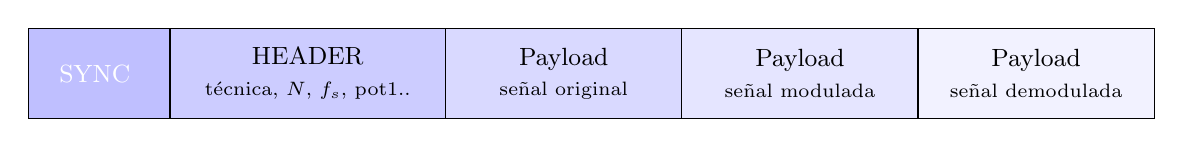
\begin{tikzpicture}[
    font=\small,
    block/.style={
        draw,
        minimum height=1.15cm,
        align=center
    }
]

\node[block, fill=blue!25, text=white, minimum width=1.8cm] (sync) at (0,0) {
SYNC
};

\node[block, fill=blue!20, minimum width=3.5cm] (header) at (2.65,0) {
HEADER\\
\scriptsize técnica, $N$, $f_s$, pot1..
};

\node[block, fill=blue!15, minimum width=3.0cm] (msg) at (5.9,0) {
Payload\\
\scriptsize señal original
};

\node[block, fill=blue!10, minimum width=3.0cm] (mod) at (8.9,0) {
Payload\\
\scriptsize señal modulada
};

\node[block, fill=blue!5, minimum width=3.0cm] (dem) at (11.9,0) {
Payload\\
\scriptsize señal demodulada
};

\end{tikzpicture}
    \caption{Estructura general propuesta para el frame serial sincronizado.}
    \label{fig:frame_structure}
\end{figure}

La principal ventaja de esta arquitectura corresponde a que permite conservar alineación temporal entre señales durante todo el proceso de adquisición y reconstrucción. Debido a que todas las representaciones pertenecientes a un mismo instante temporal son transmitidas dentro del mismo frame, la aplicación de monitoreo puede reconstruir directamente la relación entre etapas sin incorporar mecanismos adicionales de sincronización externa.

Considerando estas ventajas, se adopta el enfoque basado en frames seriales sincronizados como arquitectura principal para el sistema de adquisición y visualización. Aunque este enfoque introduce una mayor carga asociada al empaquetado y transmisión de información dentro del entorno embebido, se considera preferible concentrar parcialmente esta complejidad sobre el RP2040 con tal de preservar sincronización temporal entre señales y simplificar considerablemente el proceso de reconstrucción y monitoreo dentro de la aplicación externa.

Una vez establecida la estructura principal de transmisión, aparece un segundo problema asociado a la conmutación dinámica entre técnicas de modulación. Debido a que AM y ASK/OOK utilizan parámetros distintos y producen comportamientos diferentes sobre la interfaz de monitoreo, resulta necesario definir un mecanismo que permita identificar automáticamente cuándo ocurre un cambio de técnica dentro del sistema embebido.

Una primera alternativa consiste en incorporar un mecanismo manual de selección dentro de la propia interfaz gráfica, permitiendo que el usuario indique explícitamente cuál técnica se encuentra activa en el entorno embebido. Bajo este enfoque, el monitor reorganiza internamente sus parámetros y estructuras visuales dependiendo del estado seleccionado por el usuario, permitiendo adaptar la interfaz para representar los parámetros específicos asociados a cada técnica. La principal ventaja de esta estrategia corresponde a su simplicidad de implementación, debido a que la lógica de adquisición serial permanece prácticamente independiente del comportamiento de la interfaz. Adicionalmente, el monitor puede reorganizar directamente sus elementos visuales sin requerir información adicional proveniente del entorno embebido.

No obstante, este enfoque también introduce una dependencia directa entre el estado real del sistema embebido y la interacción manual del usuario dentro de la aplicación de monitoreo. Bajo estas condiciones, inconsistencias entre la técnica verdaderamente activa y la configuración seleccionada en la interfaz pueden provocar errores de interpretación sobre los parámetros recibidos y desalineamiento entre adquisición y visualización.

Como alternativa, se propone una arquitectura desacoplada basada en transmisión dinámica de metadata. Bajo este enfoque, el sistema embebido transmite automáticamente un paquete adicional de control cada vez que ocurre una conmutación entre técnicas. Este paquete incorpora información asociada a la técnica activa, parámetros disponibles y configuraciones requeridas para reorganizar dinámicamente el comportamiento interno del monitor.

A diferencia del frame principal de señal, cuyo objetivo consiste en transmitir muestras sincronizadas para visualización continua, el paquete de metadata se orienta a describir la configuración operativa actual del sistema. Debido a esto, el monitor puede actualizar automáticamente parámetros internos y adaptar dinámicamente su estructura cuando ocurre una conmutación entre técnicas.

La principal ventaja de esta arquitectura corresponde a que desacopla el comportamiento del monitor respecto a interacción manual del usuario y permite que la aplicación adapte automáticamente su configuración dependiendo de la técnica actualmente ejecutada. En consecuencia, la lógica de adquisición y visualización pasa a depender directamente de la información transmitida desde el entorno embebido, favoreciendo simultáneamente modularidad, sincronización y escalabilidad dentro de la arquitectura general del sistema.


\subsection{Optimización del procesamiento y flujo de datos en el sistema embebido}

La disposición de una arquitectura funcional para la ejecución continua de las técnicas de modulación y demodulación no garantiza por sí sola la estabilidad operativa del sistema embebido. Una vez establecidas las adaptaciones algorítmicas y la estructura básica de comunicación descritas en las Seccion \ref{sec:adaptacion}, la operación continua del sistema evidenció que distintos aspectos relacionados con la organización interna del procesamiento, la estructura del protocolo de transmisión serial y la parametrización del sistema requerían refinamientos adicionales para mejorar el rendimiento global bajo condiciones de operación sostenida. En consecuencia, el proceso de optimización se orienta hacia dos dimensiones: el refinamiento del flujo de procesamiento y la modularización estructural del sistema.

\label{subsec:refinamiento_flujo}
\subsubsection{Refinamiento del flujo de procesamiento y estabilidad temporal}

La arquitectura de procesamiento por bloques establecida en la Sección \ref{sec:flow_control} permite organizar el flujo interno de datos en tres etapas sucesivas: generación, modulación y demodulación, preservando simultáneamente las tres representaciones de señal dentro de buffers independientes. Sin embargo, el análisis del comportamiento operativo del sistema identificó que la organización inicial de este flujo y la estructura del frame serial podían optimizarse para reducir ineficiencias asociadas a la asignación de estructuras temporales en la secuencia de empaquetado de datos.

Un aspecto de refinamiento corresponde al manejo de los buffers internos de señal. En el diseño inicial, cada iteración del ciclo de procesamiento generaba estructuras de datos intermedias de forma independiente, sin aprovechar la posibilidad de reutilizar espacios de memoria previamente reservados. Bajo las restricciones de la plataforma embebida, esta práctica incrementa innecesariamente la presión sobre la memoria SRAM disponible y aumenta la frecuencia de operaciones de asignación dentro del ciclo de procesamiento continuo. La alternativa adoptada consiste en reservar de forma estática los buffers asociados a las tres etapas de señal desde el inicio del programa y reutilizarlos en cada iteración sin reinicialización innecesaria de estructuras. Esta decisión reduce el costo asociado a la gestión dinámica de memoria y contribuye a mantener un comportamiento temporal más predecible durante la ejecución continua.

Además del refinamiento del flujo de procesamiento, el análisis del sistema operando bajo condiciones continuas identificó factores adicionales que condicionan directamente la estabilidad temporal del procesamiento. Dos de ellos resultan especialmente determinantes: el tamaño del bloque de procesamiento $N$ y las limitaciones temporales inherentes a la ejecución de MicroPython sobre el microcontrolador RP2040.

Dentro de la arquitectura propuesta, el parámetro $N$ define la cantidad de muestras procesadas y transmitidas durante cada iteración completa del ciclo principal. En consecuencia, este parámetro controla simultáneamente la cantidad de información contenida en cada frame serial, el tamaño de los buffers internos y la frecuencia con la que el sistema debe ejecutar operaciones de generación, modulación, demodulación y transmisión hacia la aplicación de monitoreo.

La selección de $N$ representa una decisión de ingeniería con implicaciones directas sobre variables interdependientes como la latencia de visualización, la carga computacional por ciclo de procesamiento y la frecuencia de actualización de la interfaz gráfica. Debido a esta dependencia mutua, no existe un único valor universalmente óptimo, ya que el comportamiento del sistema cambia significativamente conforme varía el tamaño de bloque utilizado.

Con el fin de observar las implicaciones operativas asociadas al tamaño de bloque, la Tabla \ref{tab:comparacion_n} presenta una comparación general del comportamiento del sistema bajo escenarios de $N$ reducido y $N$ elevado.

\begin{table}[H]
\centering
\footnotesize
\caption{Implicaciones operativas asociadas al tamaño de bloque $N$}
\label{tab:comparacion_n}
\begin{tabular}{|p{4.9cm}|p{4.9cm}|p{4.9cm}|}
\hline
\textbf{Aspecto} & \textbf{$N$ reducido (64-256)} & \textbf{$N$ elevado (512-1024)} \\ \hline

Frecuencia de actualización visual &
Mayor frecuencia de actualización &
Menor frecuencia de actualización \\ \hline

Latencia percibida por el usuario &
Menor latencia &
Mayor latencia \\ \hline

Cantidad de transmisiones seriales &
Mayor cantidad de frames por segundo &
Menor cantidad de frames por segundo \\ \hline

Sobrecarga de empaquetado y sincronización &
Mayor frecuencia de operaciones administrativas &
Menor frecuencia de operaciones administrativas \\ \hline

Carga computacional instantánea por iteración &
Menor cantidad de muestras por ciclo &
Mayor cantidad de muestras por ciclo \\ \hline

Estabilidad temporal del procesamiento &
Mayor sensibilidad a variaciones temporales &
Comportamiento más uniforme \\ \hline

Capacidad de respuesta ante cambios de parámetros &
Respuesta más inmediata &
Respuesta más gradual \\ \hline

\end{tabular}
\end{table}

Como puede observarse, ambos escenarios presentan ventajas y restricciones distintas dependiendo de las prioridades operativas del sistema. Mientras valores reducidos de $N$ favorecen una respuesta visual más inmediata y una interacción más dinámica con los parámetros físicos del sistema, valores elevados permiten disminuir la frecuencia de operaciones administrativas y estabilizar parcialmente el comportamiento temporal del procesamiento continuo. Debido a ello, el tamaño de bloque no puede tratarse como un parámetro fijo universal, ya que su selección condiciona directamente el balance entre latencia, estabilidad y carga computacional dentro del entorno embebido.

MicroPython introduce además una restricción adicional sobre este balance operacional. A diferencia de implementaciones compiladas en C o C++, la ejecución interpretada incrementa la sobrecarga temporal asociada a operaciones matemáticas iterativas, empaquetado serial y manipulación continua de buffers dentro del ciclo principal. Esta condición adquiere mayor relevancia conforme aumenta la frecuencia de iteraciones requerida por bloques pequeños o la cantidad de muestras procesadas por bloques grandes.

A partir de este análisis, resulta preferible definir el tamaño de bloque $N$ como un parámetro configurable externamente, en lugar de fijarlo como una constante interna del firmware. Esta decisión permite adaptar dinámicamente el comportamiento temporal del sistema según las necesidades de operación, priorizando distintos criterios como estabilidad, latencia o capacidad de respuesta sin requerir modificaciones sobre la lógica principal de procesamiento.

\subsubsection{Optimización de modularidad estructural del sistema}

La segunda dimensión de optimización corresponde a la modularidad estructural del sistema embebido. El diseño de arquitectura inicial de la Figura \ref{fig:arquitectura} organiza el procesamiento dentro de un módulo principal complementado por módulos independientes para cada técnica implementada. Aunque esta organización resulta funcional, inicialmente no se establecía una interfaz genérica que permitiera tratar cada técnica bajo una estructura modular uniforme, por lo que la escalabilidad del sistema resultaba limitada. Bajo este enfoque, la integración de nuevas técnicas obliga a realizar modificaciones directas sobre el módulo principal de procesamiento, incrementando la complejidad de mantenimiento y el riesgo de introducir errores de integración.

El refinamiento adoptado establece una arquitectura modular basada en una interfaz genérica para los módulos de cada técnica. Bajo este esquema, cada implementación encapsula internamente sus variables de continuidad y parámetros de procesamiento, manteniendo una estructura estandarizada de interacción con el módulo principal. Esto permite desacoplar la lógica de procesamiento general de los detalles internos de cada técnica, facilitando la incorporación de nuevos módulos sin alterar la lógica central del sistema.

Otro aspecto de optimización corresponde a la parametrización externa del sistema. Debido a las decisiones de modularidad adoptadas y al refinamiento del flujo de procesamiento descrito en la Sección \ref{subsec:refinamiento_flujo}, surge la necesidad de reorganizar la gestión de configuraciones del sistema. Inicialmente, parámetros como la frecuencia de muestreo $F_s$, el tamaño de bloque $N$ y los rangos de mapeo asociados a los potenciómetros se encontraban definidos directamente dentro del firmware del microcontrolador, lo que implicaba modificar y recargar el sistema embebido ante cualquier ajuste operativo.

Como refinamiento, se incorpora un archivo de configuración en formato JSON gestionado desde la aplicación de monitoreo. Esta abstracción permite separar los parámetros de operación de la lógica de procesamiento implementada en el sistema embebido, centralizando la configuración del sistema en un único archivo externo.

La configuración se organiza en dos categorías principales: parámetros generales del sistema, como frecuencia de muestreo, tamaño de bloque, velocidad de transmisión serial y parámetros globales de operación; y parámetros específicos de cada técnica, incluyendo identificación del módulo, tipo de señal procesada y rangos de mapeo asociados a cada potenciómetro. Esta organización permite que la aplicación de monitoreo incorpore una herramienta visual de configuración capaz de modificar parámetros y regenerar automáticamente el archivo de configuración sin intervenir directamente sobre el firmware del microcontrolador.

\subsection{Implementación del proceso de evaluación y análisis de desempeño}

La disposición de un sistema funcional capaz de modular, demodular y visualizar señales en tiempo real no constituye por sí sola evidencia suficiente sobre la calidad del procesamiento realizado. La inspección visual de las formas de onda reconstruidas permite identificar anomalías groseras en el comportamiento del sistema, pero resulta insuficiente para caracterizar con precisión la fidelidad de reconstrucción, la estabilidad temporal del procesamiento y la sensibilidad del sistema ante variaciones en los parámetros de operación. Dos señales pueden mostrar formas visualmente similares y presentar, no obstante, diferencias significativas en amplitud, desplazamiento de fase o dispersión acumulada que un análisis puramente cualitativo no detecta. Por esta razón, la incorporación de un proceso de evaluación cuantitativa integrado al flujo operativo del sistema constituye uno de los principales objetivos dentro del desarrollo del proyecto.

El problema central que este objetivo aborda consiste en definir un conjunto de métricas matemáticas complementarias que permitan caracterizar el desempeño del sistema desde perspectivas distintas y no redundantes. La complementariedad es un criterio determinante en la selección: una única métrica captura solamente una dimensión del problema, por lo que combinaciones mal seleccionadas pueden producir una evaluación sesgada o incompleta. En este contexto, el diseño del sistema de evaluación requiere identificar cuáles son las dimensiones de desempeño relevantes para el problema planteado, para poder seleccionar el conjunto de métricas más adecuado para cada dimensión.

A diferencia de las etapas previas del desarrollo, donde las restricciones computacionales del entorno embebido condicionaban directamente las decisiones de diseño algorítmico, la evaluación matemática se ejecuta íntegramente dentro de la aplicación de monitoreo en el entorno de escritorio. Esta distribución resulta determinante, ya que permite emplear formulaciones con mayor precisión numérica y operaciones vectorizadas sin imponer carga adicional sobre el microcontrolador. El módulo de métricas opera sobre los bloques de señal recibidos por comunicación serial, calculando los indicadores de desempeño en cada ciclo de actualización del monitor.

\subsubsection{Selección de métricas de evaluación}

El desempeño del sistema de modulación y demodulación puede caracterizarse a partir de tres dimensiones fundamentales: la similitud global entre la señal original y la señal reconstruida, la precisión numérica de la reconstrucción punto a punto, y la estabilidad temporal del procesamiento durante la ejecución continua por bloques. Cada una de estas dimensiones exige una aproximación matemática distinta, y la selección de métricas apropiadas requiere considerar tanto las propiedades formales de las métricas candidatas como su adecuación al tipo de señal procesada y a las características del entorno de operación.

\textbf{Dimensión 1: Similitud global entre señales.} La primera dimensión busca cuantificar en qué medida la señal demodulada preserva la forma general de la señal original, con independencia de posibles diferencias de amplitud o desplazamiento en continua introducidos por el proceso de filtrado o por el acondicionamiento de la señal dentro del embebido. Para esta dimensión existen múltiples alternativas establecidas en la literatura de procesamiento de señales.

Una primera opción corresponde al coeficiente de determinación $R^2$, ampliamente utilizado en análisis de regresión como indicador de la fracción de varianza explicada por el modelo. Sin embargo, su interpretación asume una relación lineal entre las señales comparadas y es sensible a diferencias de escala absoluta, lo que lo hace menos robusto ante variaciones de amplitud sistemáticas introducidas por el procesamiento embebido \cite{kay1993fundamentals}. Una segunda alternativa corresponde a la coherencia espectral, que evalúa la similitud entre señales en el dominio de la frecuencia. Aunque esta métrica es apropiada para análisis estacionario de señales, su cálculo requiere transformadas de Fourier sobre ventanas suficientemente largas, lo que introduce latencia en la retroalimentación y resulta más adecuado para análisis post-procesado que para retroalimentación en tiempo real.

La métrica seleccionada para esta dimensión corresponde a la Correlación Cruzada Normalizada (NCC), formulada como la correlación de Pearson entre la señal original y la señal demodulada, centradas respecto a sus respectivas medias, tal como se expresa en la ecuación \ref{eq:ncc_analogico}.

\begin{equation}
\text{NCC} = \frac{\displaystyle\sum_{i=1}^{N}(x_i - \bar{x})(y_i - \bar{y})}
{\sqrt{\displaystyle\sum_{i=1}^{N}(x_i - \bar{x})^2}
\sqrt{\displaystyle\sum_{i=1}^{N}(y_i - \bar{y})^2}}
\label{eq:ncc_analogico}
\end{equation}

La elección de NCC frente a las alternativas descritas se justifica en que la normalización respecto a las normas de ambas señales hace que el resultado sea invariante ante diferencias de escala y offset, lo cual resulta especialmente relevante en este contexto dado que el procesamiento de demodulación introduce componentes de continua y variaciones de amplitud que no constituyen degradación real de la técnica sino artefactos del acondicionamiento. El resultado está acotado en $[-1, 1]$, lo que facilita su interpretación como porcentaje de similitud al escalarlo al rango $[0, 100]$, y su cálculo requiere únicamente operaciones vectoriales básicas, compatibles con una actualización por bloque en tiempo real.

No obstante, la aplicación directa de NCC sobre señales digitales presenta una limitación fundamental. En la técnica ASK/OOK, la señal original corresponde a una secuencia binaria representada en formato NRZ, por lo que la correlación analógica entre la señal original y la demodulada puede verse influenciada por la forma de los pulsos reconstituidos y no reflejar fielmente la tasa de recuperación de bits. En este caso, la métrica más informativa consiste en comparar directamente la correspondencia lógica entre ambas señales, convirtiendo ambas a representación binaria mediante umbral de signo y calculando la fracción de bits correctamente recuperados, conforme se define en la ecuación \ref{eq:ncc_digital}.

\begin{equation}
\text{NCC}_{\text{digital}} = \frac{1}{N}\sum_{i=1}^{N}
\mathbf{1}\left[\text{sgn}(x_i) = \text{sgn}(y_i)\right] \times 100
\label{eq:ncc_digital}
\end{equation}

Esta diferenciación en el cálculo de NCC según el tipo de técnica activa es esencial, ya que aplicar la correlación analógica a señales digitales introduciría una evaluación estructuralmente incorrecta. La selección automática de la variante adecuada a partir del campo de identificación de técnica contenido en los metadatos del protocolo serial garantiza que la métrica sea siempre coherente con la naturaleza de la señal procesada.

\textbf{Dimensión 2: Precisión numérica de la reconstrucción.} La segunda dimensión complementa la evaluación de similitud al medir cuán exactamente los valores de la señal demodulada coinciden con los valores de la señal original en cada instante. Una señal puede presentar alta correlación con la original ---conservando adecuadamente su forma general--- y aun así contener desviaciones sistemáticas de amplitud, errores de escala o distorsión en regiones específicas que el NCC no detecta por su naturaleza invariante a la escala.

Para esta dimensión, la alternativa más directa corresponde al Error Cuadrático Medio (RMSE), que cuantifica la raíz del error promedio cuadrático punto a punto entre ambas señales. Sin embargo, el RMSE en su forma estándar es dimensional y dependiente de la amplitud de la señal, lo que impide comparar resultados entre bloques procesados bajo diferentes configuraciones de parámetros o entre las dos técnicas implementadas, las cuales operan sobre señales con rangos dinámicos distintos. La normalización respecto al rango dinámico de la señal original resuelve esta limitación, dando lugar al Error Cuadrático Medio Normalizado (NRMSE), definido en la ecuación~\ref{eq:nrmse}.

\begin{equation}
\text{NRMSE} = \frac{\sqrt{\dfrac{1}{N}\displaystyle\sum_{i=1}^{N}(x_i - y_i)^2}}
{x_{\max} - x_{\min}}
\label{eq:nrmse}
\end{equation}

La adopción de NRMSE sobre RMSE se justifica precisamente en esta propiedad de invarianza al rango dinámico, que permite interpretar el error en términos relativos respecto a la excursión total de la señal de referencia. Adicionalmente, la implementación incorpora una etapa de compensación de desfase y ganancia previa al cálculo del error, con el propósito de desacoplar la degradación real introducida por el proceso de modulación y demodulación de los desplazamientos temporales y variaciones de amplitud asociados al filtrado pasa bajos aplicado durante la reconstrucción de la señal. De esta manera, el indicador refleja principalmente la fidelidad efectiva de reconstrucción y no distorsiones deterministas inherentes al procesamiento interno del sistema.

\textbf{Dimensión 3: Estabilidad temporal del procesamiento continuo.} Las dos métricas anteriores caracterizan el desempeño del sistema en cada bloque individualmente, pero no capturan el comportamiento del sistema a lo largo del tiempo durante la ejecución continua. En un sistema que procesa señales mediante bloques secuenciales, es posible que el desempeño sea aceptable en promedio pero que exhiba variaciones significativas entre bloques consecutivos, lo cual evidenciaría inestabilidad en el procesamiento, problemas de sincronización serial o sensibilidad excesiva a las transiciones entre bloques.

Para esta dimensión se consideró el uso de la varianza temporal del NRMSE, que mediría directamente la dispersión del error de reconstrucción a lo largo del tiempo. Sin embargo, dado que NCC ya constituye el indicador principal de calidad del sistema, resulta más informativo y coherente evaluar la estabilidad sobre la misma métrica base, manteniendo consistencia semántica en la interpretación de los indicadores. La desviación estándar del historial de valores NCC entre bloques consecutivos cumple esta función, según se expresa en la ecuación \ref{eq:std_ncc}.

\begin{equation}
\sigma_{\text{NCC}} = \sqrt{\frac{1}{M}\sum_{i=1}^{M}
\left(\text{NCC}_i - \overline{\text{NCC}}\right)^2}
\label{eq:std_ncc}
\end{equation}

donde $M$ representa la cantidad de bloques acumulados en el historial y $\overline{\text{NCC}}$ el promedio de los valores registrados. Una desviación estándar reducida indica que el desempeño del sistema se mantiene consistente entre bloques, mientras que valores elevados pueden evidenciar inestabilidad en el procesamiento, pérdida de sincronización en el protocolo serial o degradación temporal asociada a variaciones en los parámetros del embebido durante la ejecución.


\subsubsection{Integración dentro del flujo operativo del monitor}

La integración de las métricas dentro del sistema de monitoreo requiere definir en qué punto del flujo de adquisición y visualización se realiza su cálculo, con qué periodicidad se actualizan y de qué forma se vinculan con los datos transmitidos por el embebido. Dado que el sistema recibe bloques de señal en forma continua y el protocolo serial transmite en cada frame las tres versiones sincronizadas de la señal, resulta natural vincular el cálculo de métricas directamente al evento de recepción de un nuevo frame, de forma que cada bloque procesado genere automáticamente una actualización de los indicadores de desempeño.

Bajo este esquema, por cada frame recibido el sistema extrae los vectores correspondientes a la señal original y la señal demodulada, selecciona la variante de NCC adecuada según el tipo de técnica activa identificado en los metadatos del frame, y registra el resultado en el historial de bloques para el posterior cálculo de la desviación estándar. La decisión de realizar el cálculo sobre el bloque más recientemente recibido, en lugar de acumular múltiples bloques en un buffer extendido, responde a la necesidad de mantener retroalimentación en tiempo real sin introducir latencia adicional en el ciclo de actualización de la interfaz. El historial de valores NCC se conserva internamente como una ventana deslizante, permitiendo calcular $\sigma_{\text{NCC}}$ sobre la ventana acumulada sin requerir almacenamiento indefinido de señales pasadas.

En conjunto, la implementación de este proceso de evaluación proporciona al sistema un mecanismo de retroalimentación cuantitativa que complementa la visualización gráfica de señales y permite caracterizar objetivamente el comportamiento del sistema bajo distintas configuraciones de parámetros, técnicas activas y condiciones de operación del entorno embebido.


\section{Análisis de los resultados obtenidos}

\subsection{Resultados asociados a la integración de los algoritmos de modulación y demodulación}

La evaluación funcional de las técnicas implementadas se realizó mediante pruebas variando sistemáticamente los parámetros de control disponibles en el sistema físico. El objetivo de estas pruebas consiste en observar cómo los cambios de configuración afectan la profundidad de modulación, la calidad de reconstrucción de la señal, verificando simultáneamente que el sistema mantiene operación continua y estable bajo distintas condiciones.

\subsubsection{Resultados obtenidos para la técnica AM}

Para la técnica AM, las pruebas se realizaron variando el índice de modulación $\mu$ a lo largo del rango disponible, con el propósito de observar su efecto sobre la profundidad de envolvente, la estabilidad visual de la señal modulada y la calidad de reconstrucción de la señal demodulada. Los resultados obtenidos para tres valores representativos de $\mu$ se presentan a continuación.

\begin{figure}[H]
\centering
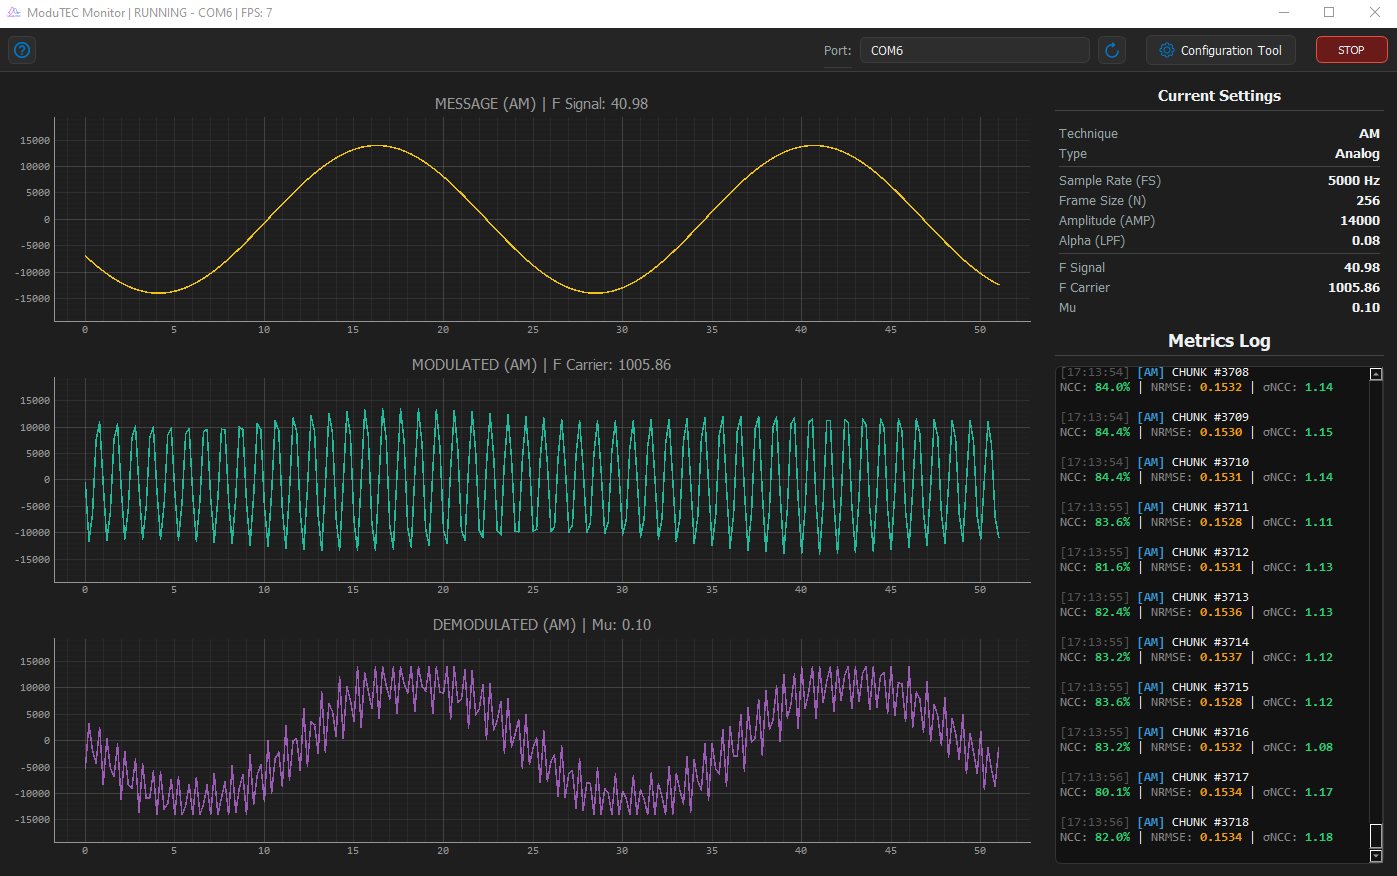
\includegraphics[width=0.74\textwidth]{fig/am-3.png}
\caption{Resultados obtenidos para AM utilizando $\mu = 0.10$. Fuente: Elaboración propia.}
\label{fig:am_mu010}
\end{figure}

La Figura \ref{fig:am_mu010} muestra el comportamiento del sistema para un índice de modulación reducido ($\mu = 0.10$). En este caso, la profundidad de modulación sobre la envolvente es baja, lo que se traduce en una variación de amplitud poco pronunciada sobre la señal modulada. Como consecuencia directa, la señal demodulada presenta una mayor presencia de componentes residuales asociadas a la portadora, las cuales no son completamente suprimidas por el filtro pasa bajos de primer orden utilizado. Este comportamiento es consistente con la decisión de diseño que priorizó simplicidad computacional sobre selectividad frecuencial del filtrado: a bajos índices de modulación, la energía de la componente de información es proporcionalmente menor respecto a la portadora, lo que reduce la efectividad relativa del filtrado recursivo empleado. Los valores de NCC registrados se sitúan en el rango de 82--84\%, indicando que la forma general de la señal es recuperada, si bien con menor similitud respecto a configuraciones de mayor profundidad. El NRMSE observado alcanza valores alrededor de 0.15, reflejando el efecto del residuo de alta frecuencia sobre el error punto a punto. No obstante, el sistema mantiene funcionamiento continuo y estable, sin evidenciar pérdida de sincronización ni interrupciones en el flujo de procesamiento.

\begin{figure}[H]
\centering
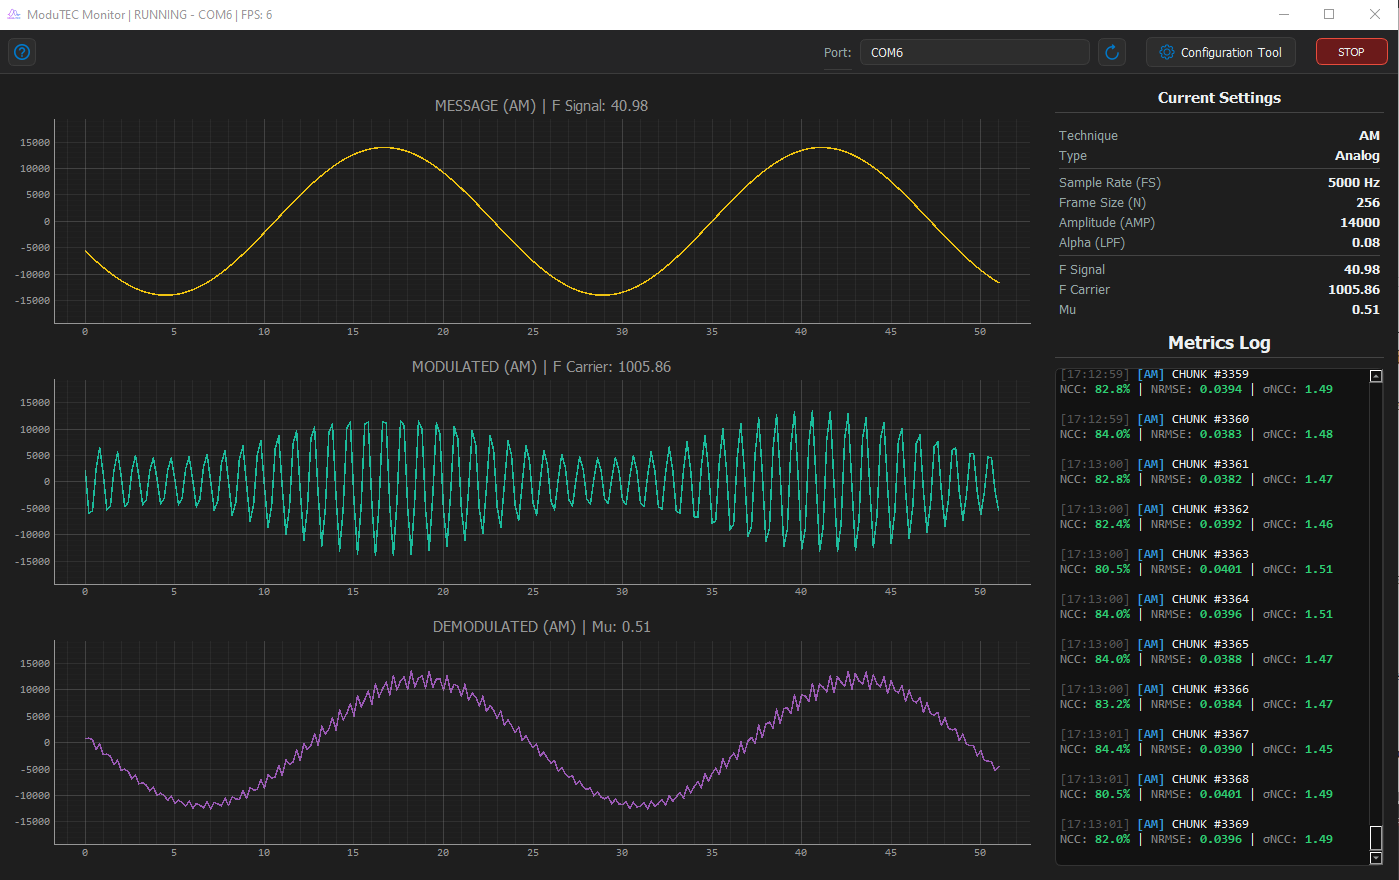
\includegraphics[width=0.74\textwidth]{fig/am-2.png}
\caption{Resultados obtenidos para AM utilizando $\mu = 0.51$. Fuente: Elaboración propia.}
\label{fig:am_mu051}
\end{figure}

Al incrementar el índice de modulación a un valor intermedio ($\mu = 0.51$), los resultados presentados en la Figura \ref{fig:am_mu051} evidencian una mejora notable en la calidad de reconstrucción. La mayor profundidad de modulación incrementa la relación entre la energía de la señal de información y la portadora, lo que favorece la supresión de componentes residuales durante el filtrado y permite que la señal demodulada conserve con mayor fidelidad la forma de onda original. El NCC se mantiene en el rango de 82--84\%, aunque la reducción del NRMSE hacia valores de 0.03--0.04 evidencia que el error de reconstrucción punto a punto disminuye sustancialmente respecto al caso anterior. Este resultado indica que, si bien la similitud de forma general se preserva en ambas configuraciones, la modulación intermedia produce un equilibrio más favorable entre estabilidad visual y precisión de reconstrucción.

\begin{figure}[H]
\centering
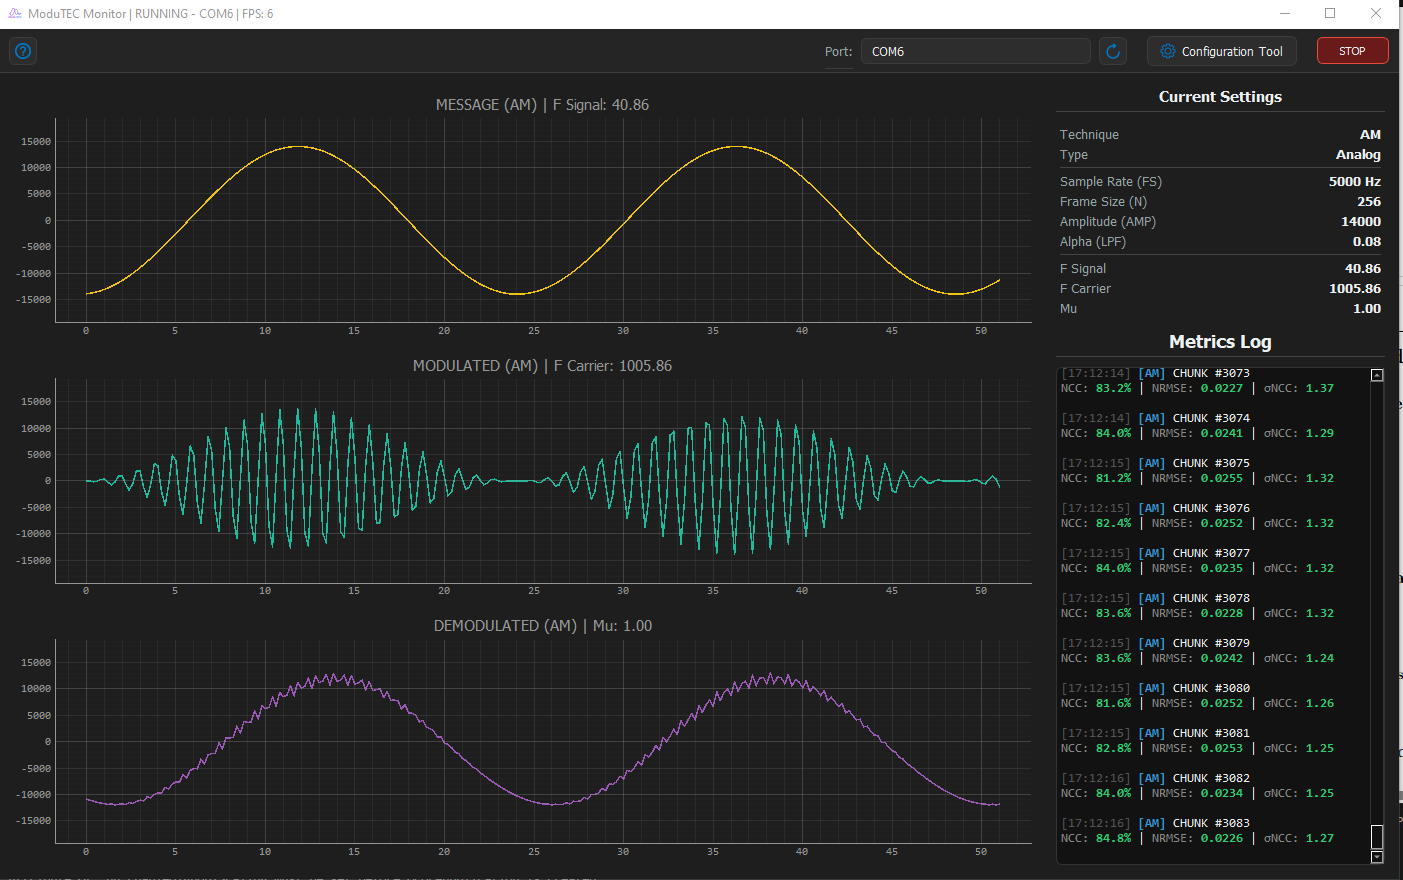
\includegraphics[width=0.74\textwidth]{fig/am-1.png}
\caption{Resultados obtenidos para AM utilizando $\mu = 1.00$. Fuente: Elaboración propia.}
\label{fig:am_mu100}
\end{figure}

La Figura \ref{fig:am_mu100} presenta los resultados obtenidos para máxima profundidad de modulación ($\mu = 1.00$). En esta configuración, la envolvente de la señal modulada se encuentra claramente definida, y la señal demodulada presenta la mayor aproximación visual a la señal original observada durante las pruebas. El NRMSE alcanza valores extremadamente bajos, en torno a 0.02, lo que confirma que el incremento de $\mu$ reduce significativamente el error de reconstrucción al maximizar la profundidad de la componente de información dentro de la señal modulada. El sistema conserva sincronización continua entre generación, modulación y demodulación, sin evidenciar inestabilidad temporal incluso bajo la mayor carga de modulación evaluada. Este resultado valida que la formulación discreta simplificada adoptada para la técnica AM es capaz de sostener una reconstrucción de alta calidad dentro del entorno embebido cuando el índice de modulación opera en su valor máximo.

La comparación entre las tres configuraciones evaluadas muestra que el índice de modulación constituye el factor determinante sobre la calidad de reconstrucción en AM: valores bajos de $\mu$ introducen mayor residuo de portadora y elevan el error de reconstrucción, mientras que valores intermedios y altos permiten reducir el NRMSE de forma significativa sin comprometer la estabilidad operativa del sistema. En conjunto, los resultados confirman que la técnica AM logra ejecutarse correctamente sobre el RP2040 bajo distintas configuraciones de parámetros, manteniendo funcionamiento continuo y recuperación funcional de la señal en todos los casos evaluados.


% =========================================================
\subsubsection{Resultados obtenidos para la técnica ASK/OOK}

Para la técnica ASK/OOK, las pruebas se orientaron a evaluar la estabilidad de la recuperación binaria ante variaciones en la secuencia digital generada y ante cambios en el umbral de decisión $\tau$. Dado que la naturaleza de la señal procesada es discreta, el comportamiento del sistema se analiza en términos de coherencia entre los patrones de activación y desactivación de la portadora observados en la señal modulada y la correspondencia lógica entre la señal original y la señal demodulada.

\begin{figure}[H]
\centering
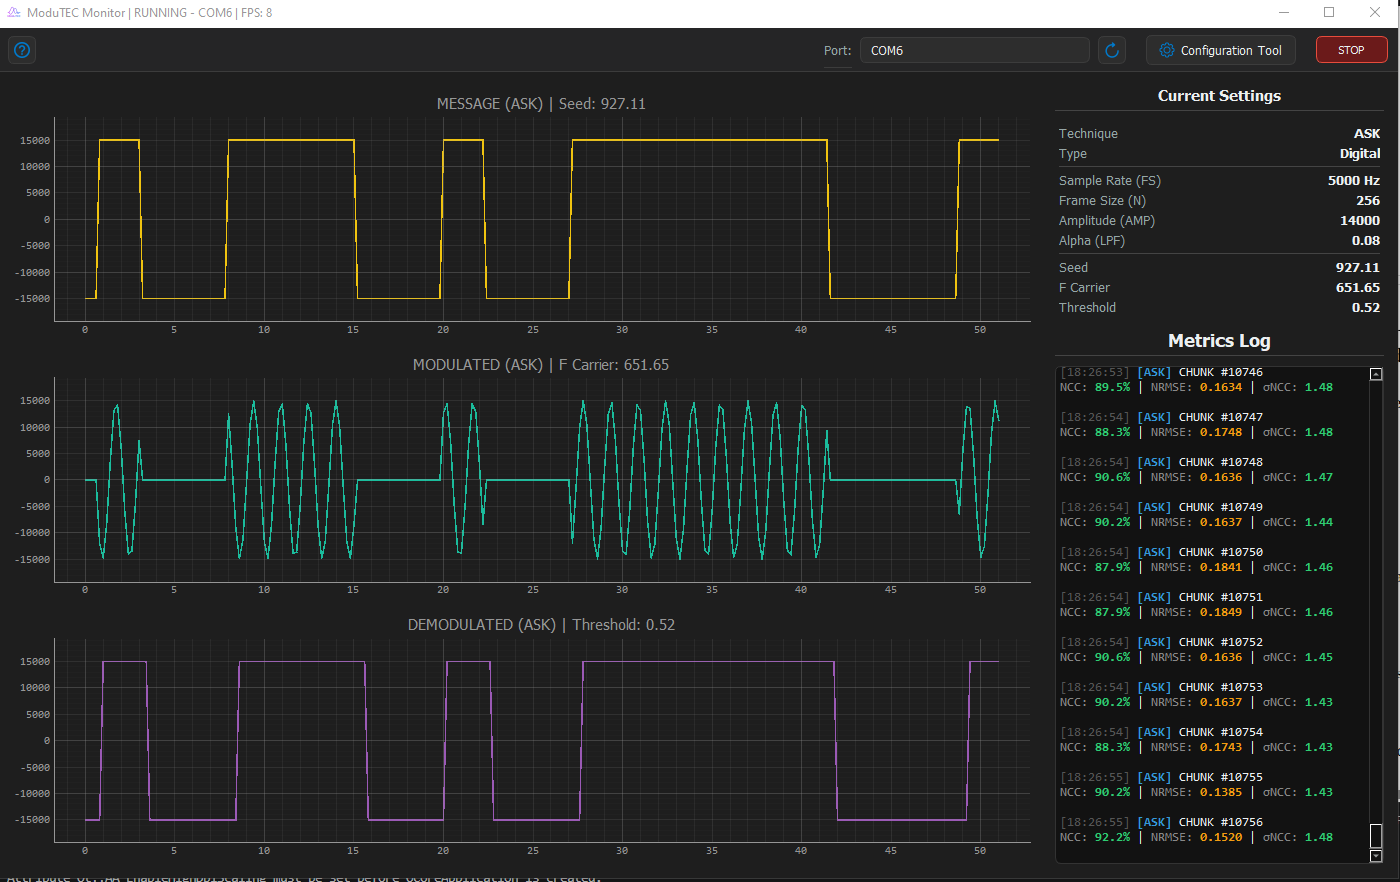
\includegraphics[width=0.74\textwidth]{fig/ask-1.png}
\caption{Resultados obtenidos para ASK/OOK con $\tau = 0.52$. Fuente: Elaboración propia.}
\label{fig:ask_th052}
\end{figure}

La Figura \ref{fig:ask_th052} muestra el comportamiento del sistema bajo un umbral de decisión cercano al valor central del rango normalizado ($\tau = 0.52$). En esta configuración, la activación y desactivación de la portadora refleja fielmente los estados lógicos generados por el mecanismo pseudoaleatorio, y la coincidencia visual entre la señal original y la señal demodulada es notoria. Los valores de NCC digital registrados se sitúan en el rango de 88--92\%, evidenciando que el sistema recupera correctamente la mayor parte de los bits transmitidos. El NRMSE se ubica en el rango de 0.15--0.18, valor que es esperable para señales de naturaleza binaria, ya que la métrica es sensible a las transiciones abruptas características de este tipo de señal. La estabilidad temporal entre bloques consecutivos es adecuada, sin evidencia de desalineamiento entre la secuencia generada y la recuperada.

\begin{figure}[H]
\centering
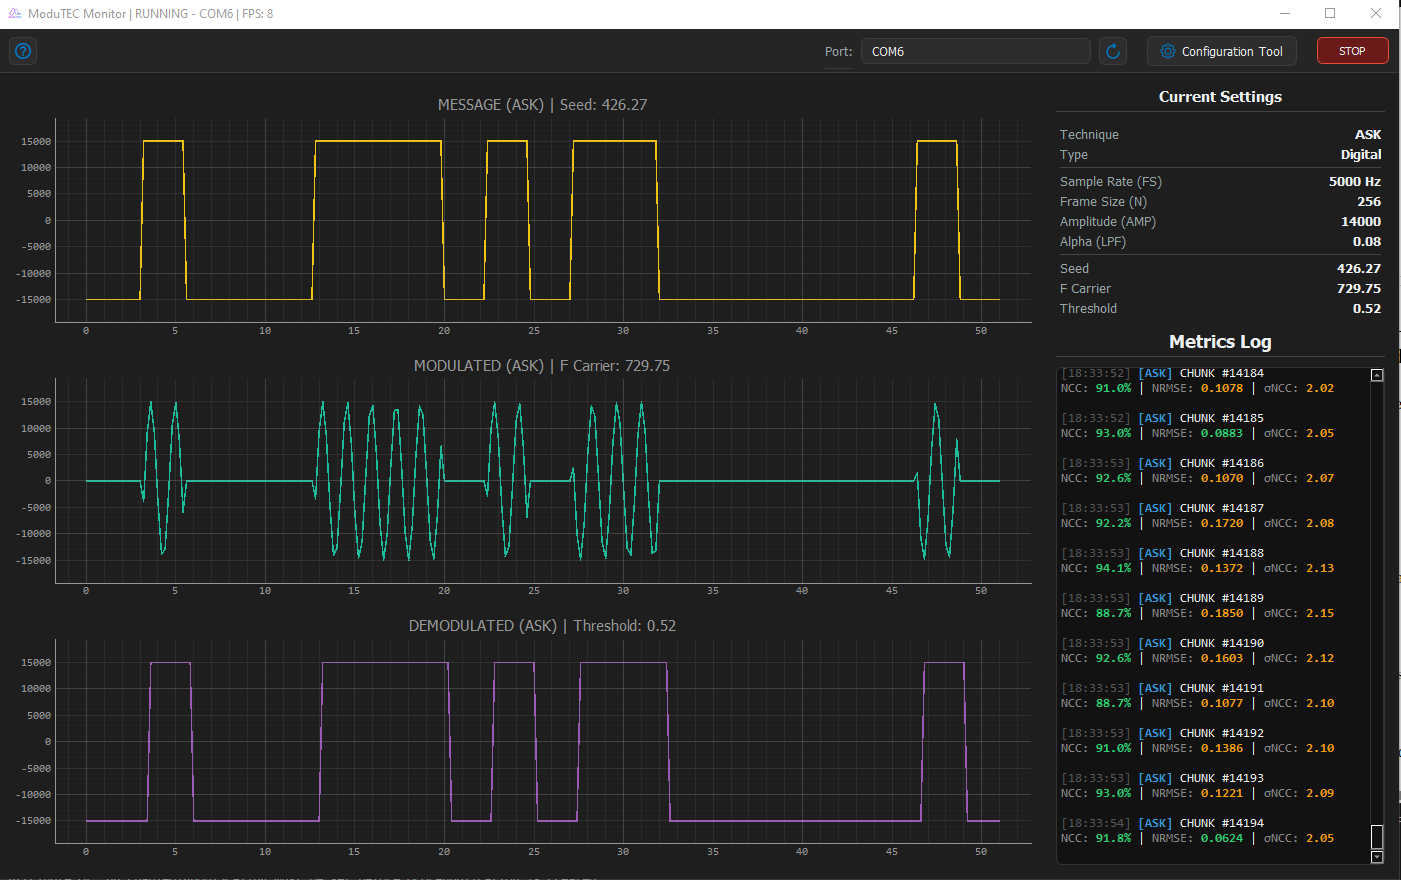
\includegraphics[width=0.74\textwidth]{fig/ask-2.png}
\caption{Resultados obtenidos para ASK/OOK con una secuencia digital distinta. Fuente: Elaboración propia.}
\label{fig:ask_seed2}
\end{figure}

Con el propósito de evaluar si la estabilidad del sistema depende de un patrón binario específico, la Figura \ref{fig:ask_seed2} presenta los resultados obtenidos al modificar el valor de semilla del generador pseudoaleatorio, produciendo una secuencia digital diferente. El cambio en el patrón binario es visible en la señal modulada, que presenta una distribución distinta de bloques activos e inactivos respecto al caso anterior. Sin embargo, el comportamiento del sistema en términos de recuperación binaria se mantiene estable, con NCC digital en el rango de 89--93\%. En algunos bloques evaluados, el NRMSE desciende hasta valores de 0.06, asociados a secuencias con menor densidad de transiciones. Este resultado confirma que la sincronización del sistema no depende de características particulares de la secuencia transmitida, sino que se mantiene de forma consistente independientemente del patrón generado.

\begin{figure}[H]
\centering
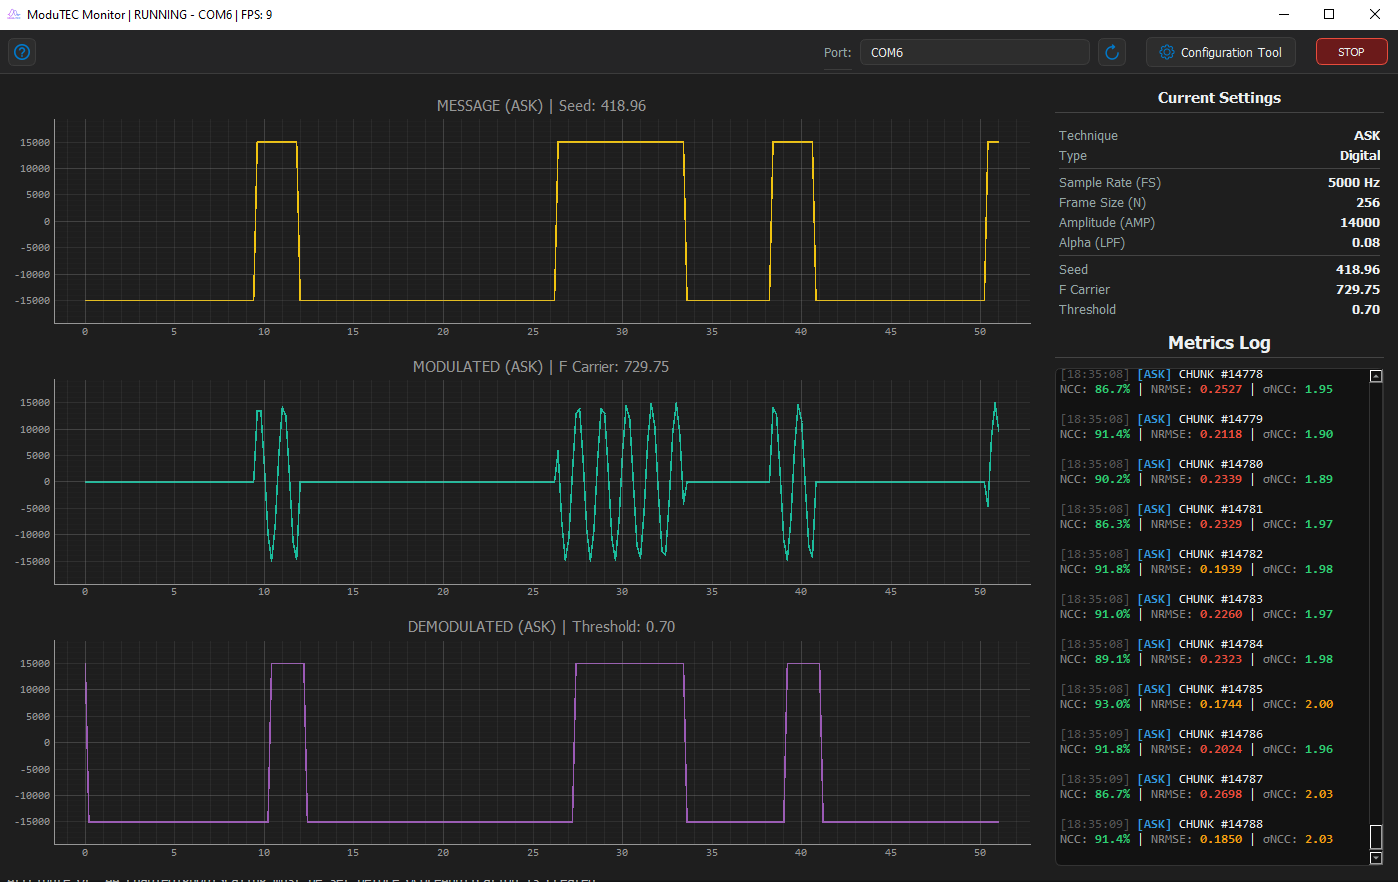
\includegraphics[width=0.74\textwidth]{fig/ask-3.png}
\caption{Resultados obtenidos para ASK/OOK con $\tau = 0.70$. Fuente: Elaboración propia.}
\label{fig:ask_th070}
\end{figure}

La Figura \ref{fig:ask_th070} evidencia el efecto de incrementar el umbral de decisión hacia un valor más alto ($\tau = 0.70$). En esta configuración, el proceso de detección binaria se vuelve más exigente, ya que una fracción mayor de los valores detectados debe superar el umbral para ser interpretados como estado lógico activo. Como consecuencia, la sensibilidad del detector aumenta y el error de reconstrucción se eleva, con valores de NRMSE en el rango de 0.20--0.25. Este incremento refleja que algunos bits cuya componente detectada se sitúa entre 0.52 y 0.70 son ahora clasificados incorrectamente, degradando la correspondencia lógica entre la señal original y la recuperada. Pese a este incremento en el error, el sistema conserva operación continua y estable, sin interrupciones en el procesamiento ni pérdida de sincronización serial.

El análisis comparativo entre las configuraciones evaluadas para ASK/OOK muestra que el umbral de decisión constituye el principal factor de sensibilidad del proceso de recuperación binaria: valores cercanos al punto central del rango producen la mejor tasa de recuperación, mientras que umbrales más alejados incrementan el error de clasificación. Adicionalmente, la variación de la secuencia digital no compromete la estabilidad del sistema, confirmando que la arquitectura de detección coherente simplificada adoptada mantiene su efectividad con independencia del patrón binario transmitido. En conjunto, los resultados confirman que la técnica ASK/OOK logra recuperar correctamente la información digital bajo las distintas configuraciones evaluadas, evidenciando el funcionamiento correcto del sistema para esta modalidad de modulación.


% =========================================================
\subsection{Resultados asociados al sistema de visualización y monitoreo}

Las Figuras \ref{fig:am_mu010} a \ref{fig:ask_th070} presentadas en la subsección anterior no solo documentan el comportamiento de las técnicas de modulación y demodulación, sino que constituyen simultáneamente evidencia directa del funcionamiento del sistema de visualización y monitoreo desarrollado. En cada una de estas figuras es posible observar la representación simultánea de la señal original, la señal modulada y la señal demodulada dentro de una misma interfaz gráfica, manteniendo alineación temporal entre las tres etapas del procesamiento.

El monitor opera de forma continua durante toda la ejecución del sistema, recibiendo frames seriales sincronizados y actualizando las representaciones gráficas en cada ciclo de adquisición. La estabilidad visual observada a lo largo de las pruebas confirma que la arquitectura de visualización basada en PyQtGraph sostiene el refresco continuo de múltiples curvas sin degradar perceptiblemente el rendimiento del sistema. Adicionalmente, la interfaz integra la visualización de parámetros activos y métricas calculadas en tiempo real, permitiendo correlacionar de forma directa los cambios de configuración física con el comportamiento cuantitativo del sistema.


% =========================================================
\subsection{Resultados asociados a la optimización del procesamiento y flujo de datos}


% =========================================================
\subsubsection{Resultados del procesamiento por bloques}

Con el propósito de determinar el tamaño de bloque más adecuado para la operación del sistema, se evaluó el comportamiento del procesamiento bajo distintos valores de $N$, observando el impacto sobre la frecuencia de actualización visual, la estabilidad temporal del procesamiento y la latencia percibida durante la ejecución continua. La Tabla \ref{tab:comparacion_fps_n} resume el comportamiento observado para los valores de $N$ evaluados.

\begin{table}[H]
\centering
\caption{Comportamiento del sistema bajo distintos tamaños de bloque $N$.}
\label{tab:comparacion_fps_n}
\resizebox{0.8\textwidth}{!}{
\begin{tabular}{|>{\centering\arraybackslash}p{2cm}|>{\centering\arraybackslash}p{3cm}|>{\centering\arraybackslash}p{7cm}|>{\centering\arraybackslash}p{4cm}|}
\hline
\textbf{$N$ (muestras)} & \textbf{FPS promedio} & \textbf{Estabilidad visual} & \textbf{Latencia observada} \\ \hline
64  & 11-13 & Baja, con fluctuaciones visibles & Muy baja \\ \hline
128 & 8-10 & Moderada, con variaciones ocasionales & Baja \\ \hline
256 & 6-8 & Adecuada, comportamiento uniforme & Moderada \\ \hline
512 & 4-5 & Alta, sin fluctuaciones apreciables & Alta \\ \hline
1024 & 2-3 & Alta, muy estable & Muy alta \\ \hline
\end{tabular}
}
\end{table}

El comportamiento registrado por el medidor de FPS integrado en la aplicación de monitoreo confirma que el incremento de $N$ reduce progresivamente la frecuencia de actualización y mejora la estabilidad visual, por lo que $N = 256$ fue seleccionado como configuración operativa al representar el equilibrio más adecuado entre actualización, estabilidad y latencia, siendo además la configuración utilizada en las Figuras \ref{fig:am_mu010} a \ref{fig:ask_th070}.

% =========================================================


\subsubsection{Resultados de modularidad y parametrización}

La Figura \ref{fig:config_tool} muestra la herramienta de configuración que facilita la separación entre los parámetros generales del sistema y los parámetros específicos de cada técnica, permitiendo modificar la configuración sin afectar el firmware del microcontrolador.

\begin{figure}[H]
\centering
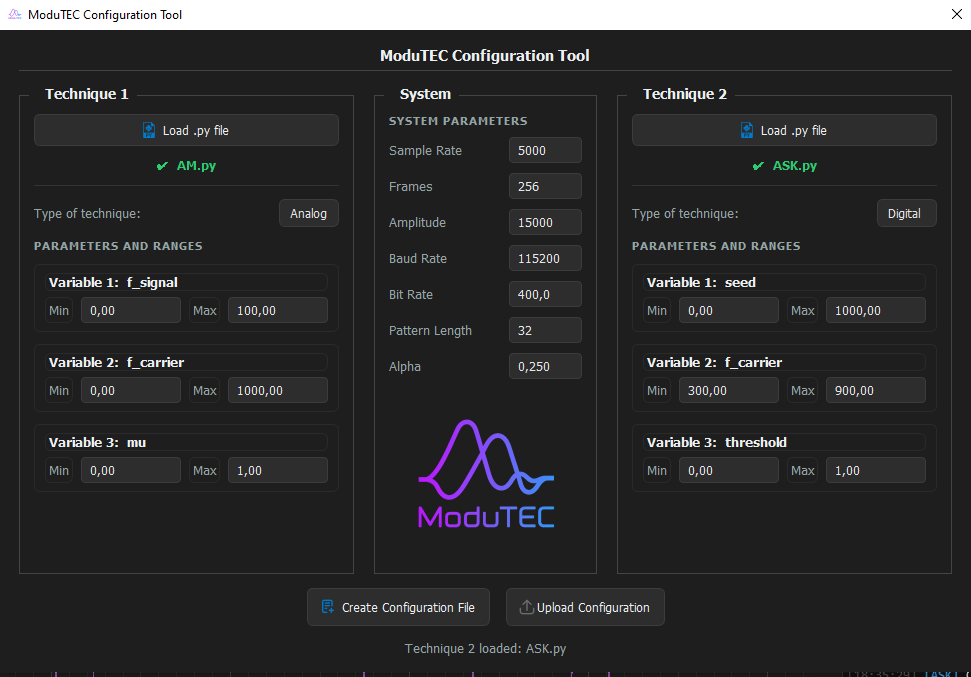
\includegraphics[width=0.75\textwidth]{fig/config-tool.png}
\caption{Herramienta de configuración desarrollada para la parametrización dinámica del sistema. Fuente: Elaboración propia.}
\label{fig:config_tool}
\end{figure}


Esta separación entre lógica de procesamiento y configuración operativa constituye un resultado directo de la arquitectura modular adoptada durante el desarrollo. La herramienta evidencia que el sistema permite incorporar nuevas técnicas de modulación y demodulación únicamente mediante la extensión del archivo de configuración y la adición del módulo correspondiente, sin necesidad de modificar el núcleo de procesamiento.

% =========================================================
\subsection{Resultados asociados al proceso de evaluación y análisis de desempeño}

Los indicadores cuantitativos calculados durante las pruebas permiten complementar el análisis visual con una caracterización objetiva del desempeño del sistema. La Tabla \ref{tab:metricas_consolidadas} resume los valores de NCC, NRMSE y $\sigma_{\text{NCC}}$ registrados para cada técnica y configuración evaluada, relacionando las tres dimensiones de desempeño dentro de una visión consolidada.

\begin{table}[H]
\centering
\caption{Resumen consolidado de métricas de desempeño por técnica y configuración.}
\label{tab:metricas_consolidadas}
\resizebox{0.9\textwidth}{!}{
\begin{tabular}{|>{\centering\arraybackslash}p{2.8cm}|>{\centering\arraybackslash}p{4.5cm}|>{\centering\arraybackslash}p{3.2cm}|>{\centering\arraybackslash}p{3.2cm}|>{\centering\arraybackslash}p{3.2cm}|}
\hline
\textbf{Técnica} & \textbf{Configuración} & \textbf{NCC promedio (\%)} & \textbf{NRMSE promedio} & \textbf{$\sigma_{\text{NCC}}$ (\%)} \\ \hline
AM & $\mu = 0.10$ & 82--84 & $\sim$0.15      & \multirow{3}{*}{$\sim$1.5--2.5} \\ \cline{1-4}
AM & $\mu = 0.51$ & 82--84 & $\sim$0.03--0.04 & \\ \cline{1-4}
AM & $\mu = 1.00$ & 83--85 & $\sim$0.02       & \\ \hline
ASK/OOK & $\tau = 0.52$, secuencia base   & 88--92 & $\sim$0.15--0.18 & \multirow{2}{*}{$\sim$1.0--2.0} \\ \cline{1-4}
ASK/OOK & $\tau = 0.52$, secuencia alterna & 89--93 & $\sim$0.06--0.15 & \\ \hline
ASK/OOK & $\tau = 0.70$ & 85--89 & $\sim$0.20--0.25 & $\sim$2.5--3.5 \\ \hline
\end{tabular}
}
\end{table}

Los valores de la Tabla \ref{tab:metricas_consolidadas} evidencian que NCC y NRMSE permiten evaluar dimensiones distintas y complementarias del desempeño, ya que mientras el NCC en AM se mantiene relativamente estable, el NRMSE varía significativamente con $\mu$, reflejando diferencias en precisión de amplitud; para ASK/OOK, los mayores valores de NCC obtenidos validan la utilización de una variante de cálculo orientada a comparación lógica binaria, mientras que los bajos valores de $\sigma_{\text{NCC}}$ en ambas técnicas confirman estabilidad temporal consistente entre bloques consecutivos.